\documentclass[11pt,a4paper,twoside]{tesis}
% \documentclass[11pt,a4paper]{tesis}

\usepackage{graphicx}
\usepackage[utf8]{inputenc}
\usepackage[spanish]{babel}
\usepackage[left=2cm,right=2cm,bottom=3.5cm,top=3.5cm]{geometry}
\usepackage{epigraph}
\usepackage{float}
\usepackage{titlesec}
\usepackage{upgreek}
\usepackage{url}
\usepackage{caption}
\usepackage{subcaption,mwe}
\usepackage{longtable}
\usepackage{amsmath}
% \usepackage{textopo}



% \usepackage{todonotes}
% \usepackage[obeyFinal]{easy-todo}
\usepackage{xcolor}
\newcommand\todo[1]{\textcolor{red}{#1}}

\begin{document}

%%%% CARATULA
\def\titulo{Licenciado}
\def\autor{Martín Ezequiel Langberg}
\def\tituloTesis{Predicción de patogenicidad en polimorfismos de un sólo nucleótido usando Aprendizaje Automático}
\def\runtitulo{Predicción de patogenicidad en polimorfismos de un sólo nucleótido usando aprendizaje automático}
\def\director{Ariel Berenstein}
\def\codirector{Pablo Turjanski}
\def\lugar{Buenos Aires, 2018}
\newcommand{\HRule}{\rule{\linewidth}{0.2mm}}
%
\thispagestyle{empty}

\begin{center}\leavevmode

\vspace{-2cm}

\begin{tabular}{l}

\includegraphics[width=2.6cm]{logofcen.pdf}
\end{tabular}


{\large \sc Universidad de Buenos Aires

Facultad de Ciencias Exactas y Naturales

Departamento de Computaci\'on}

\vspace{6.0cm}

%\vspace{3.0cm}
%{
%\Large \color{red}
%\begin{tabular}{|p{2cm}cp{2cm}|}
%\hline
%& Pre-Final Version: \today &\\
%\hline
%\end{tabular}
%}
%\vspace{2.5cm}

\begin{huge}
\textbf{\tituloTesis}
\end{huge}

\vspace{2cm}

{\large Tesis de Licenciatura en Ciencias de la Computaci\'on}

\vspace{2cm}

{\Large \autor}

\end{center}

\vfill

{\large

{Director: \director}

\vspace{.2cm}

{Codirector: \codirector}

\vspace{.2cm}

\lugar
}

\newpage\thispagestyle{empty}


%%%% ABSTRACTS, AGRADECIMIENTOS Y DEDICATORIA
\frontmatter
\pagestyle{plain}
%\begin{center}
%\large \bf \runtitulo
%\end{center}
%\vspace{1cm}
\chapter*{\runtitulo}

\noindent La predicción de enfermedades causadas por los polimorfismos de un solo nucleótido (SNPs, por sus siglas en inglés) tuvo un desarrollo constante y acelerado en los últimos años en parte gracias a nuevas técnicas de secuenciación del genoma, que permite el análisis del material genético de pacientes con mayor facilidad. Nuestro objetivo es generar un método de predicción propio a través del análisis de distintas herramientas ya existentes, reutilizando sus features más importantes, como así también agregando nuevos y explorando distintos métodos de Aprendizaje Automático que superen las métricas alcanzadas por los trabajos previos en el área.

\bigskip

\noindent\textbf{Palabras claves:} Aprendizaje Automático, Bioinformática, SNPs, Patogenicidad, Genética.

% \cleardoublepage
% %\begin{center}
%\large \bf \runtitle
%\end{center}
%\vspace{1cm}
\chapter*{\runtitle}

\noindent 

\bigskip

\noindent\textbf{Keywords:} . % OPCIONAL: comentar si no se quiere

% \cleardoublepage
% \chapter*{Agradecimientos}

Haber terminado esta Tesis de Licenciatura no solamente significó la culminación de un arduo período de trabajo sino que también representa el ``cierre'' formal de una etapa. Esto me invita a la reflexión sobre los momentos transitados durante todos estos años. 

Este trabajo no hubiera podido realizarse sin el acompañamiento recibido de muchas personas en diferentes momentos, y quiero aprovechar esta oportunidad para agradecer a todas aquellas que mi memoria me ayuda a recordar.  

A mi familia: Mis padres, hermanos, tíos, primos y abuelos. Gracias por el apoyo y el amor recibido. Especialmente a mi abuela Nelly y a mi abuela Rechel, que ya no están. Fueron mis primeras profesoras y el amor infinito que me dieron es algo que me acompaña y me da fuerzas todos los días. Se que se alegrarían muchísimo por este logro. 

A mi primer grupo de amigos durante la cursada del CBC: A Lucas y a Diego. Recuerdo con mucha felicidad haberlos tenido como compañeros en ese primer paso. Si bien después nuestros caminos se separaron, fue muy importante ese primer año de temores y éxitos compartidos.

A mis amigos eternos del secundario: Javier y Nico. Horas y horas de batallas épicas, y de campeonatos mundiales. Juntarme con ustedes siempre es el escape perfecto a otros mundos. 

A mis compañeros Mezzeteros: Ari, Javi y Gabi. Fue muy divertido haber compartido tantas materias y trabajos prácticos, pero lo mejor fue nuestro primer trabajo. Cuando llegamos a la entrevista nos confundieron con una banda de rock, y lo que siguió después fue igual de bizarro. Seguimos riéndonos de ese momento en que soñamos con ser los nuevos rockstars de la tecnología.

A mis queridos Pepes: Guille, Fixman, Luigi, Diego y JP. Estoy muy feliz y orgulloso de haber aprendido con ustedes y sobre todo de ustedes. Cómo olvidar las incontables noches comiendo pizza en el bar de deportes. Se que tengo un hogar en cualquier lugar del mundo en donde se encuentren. Quiero recordar a Leopoldo también, por haberme dado un empujón de confianza en un par de momentos importantes. Gracias, Leo.

A mis amigos del trabajo: Maxi, Yani, Pedro y Nico. Son una gran razón de mis risas durante el día a día. 

A mi gran amigo y hermano del alma Dami: Por tantas caminatas random, por los viajes y por estar siempre.

También quiero agradecer a mis directores Pablo y Ariel por todas las juntadas, por las ideas y la buena onda. En especial a Ariel por haber sido el ideólogo oficial detrás de esta ``fuga'' universitaria y en especial a Pablo por sus Vauquitas. 
Por último pero no menos importante, a la educación pública y a sus docentes por haberme acogido en cada de mis etapas de aprendizaje, me siento privilegiado y en deuda por haberme enseñado no solamente conceptos técnicos, también me ayudó a tener una conciencia social y un pensamiento crítico que me va a acompañar toda la vida.














 % OPCIONAL: comentar si no se quiere

% \cleardoublepage
% \hfill \textit{A mi persona favorita.}
  % OPCIONAL: comentar si no se quiere

% \cleardoublepage
% \tableofcontents

\mainmatter
\pagestyle{headings}

%%%% ACA VA EL CONTENIDO DE LA TESIS

% \chapter{Introducción}
% \label{ch:introduccion}
% \section{Problema biológico}

La biología, y en particular la genética, han tenido un lugar destacado en el siglo XX gracias a enormes avances como el descubrimiento de la estructura molecular del ADN, con el aporte de Franklin  \cite{FRANKLIN1953}; y Crick y Watson \cite{WATSON1953}. A partir de esos hitos científicos, se sucedieron grandes esfuerzos a nivel internacional, como el Proyecto Genoma Humano \cite{Consortium2001} o ENCODE \cite{Consortium2012}, que tienen como objetivo general el mapeo entre código genético humano y sus elementos funcionales. Estos trabajos, sumados a los recientes avances en las tecnologías de secuenciación masiva, han generado un creciente volumen de datos genómicos que a su vez favorecieron la aparición de nuevos tipos de tratamientos en el área de la medicina personalizada \cite{doi:10.1056/NEJMp1006304}. 

La medicina personalizada o de precisión es un modelo médico en donde las intervenciones se realizan a individuos o a grupos en riesgo a diferencia del modelo tradicional que apunta a la población en general. \textbf{Dentro de este área, uno de los objetivos críticos que se busca resolver es la detección de variaciones genéticas que deriven en enfermedades}.

\subsection{El dogma central de la biología}

El genoma humano está compuesto por el ADN (ácido desoxirribonucleico), que se encuentra en los 23 pares de cromosomas (moléculas de ADN) y en las mitocondrias, en las que existe una molécula de ADN denominada ADN mitocondrial. El ADN se compone de 4 bases: Adenina, Timina, Citosina, y Guanina. Estas bases se representan con su letra inicial: A, T, C y G. Cada una de estas bases está unida a otra (Adenina-Timina y Citosina-Guanina) formando pares de bases en forma helicoidal. A su vez estas cadenas pueden ser divididas en genes, que son regiones del ADN que codifican funciones. El conjunto de genes de un organismo es lo que se conoce como el genoma.

Para entender un poco cómo funciona el proceso por el cual la información genética se expresa en el organismo recurrimos al llamado "Dogma central de la biología", esbozado por Francis Crick en 1958 \cite{CRICK1958} y revisado en 1970 \cite{CRICK1970}. Este dogma, si bien fue ampliado a lo largo del tiempo, explica de forma general este proceso. Como vemos en la figura \ref{fig:esquema_dogma}, el ADN (ácido desoxirribonucleico) se transcribe en forma de ARN para luego formar una proteína. El ARN (ácido ribonucleico), es una mólecula polimérica, al igual que el ADN, y también posee las mismas bases que el ADN, excepto la timina (T) que se reemplaza por el uracilo (U). Finalmente, el ARN es utilizado para unir los aminoácidos que forman la secuencia proteica, en un proceso denominado Traducción. La secuencia del ARN se compone de tripletes adyacentes de bases que se denominan codones, y cada aminoácido está codificado por uno de estos codones (ver figura \ref{fig:table_codon}). 

\newpage

\begin{figure}[H]
\centering
    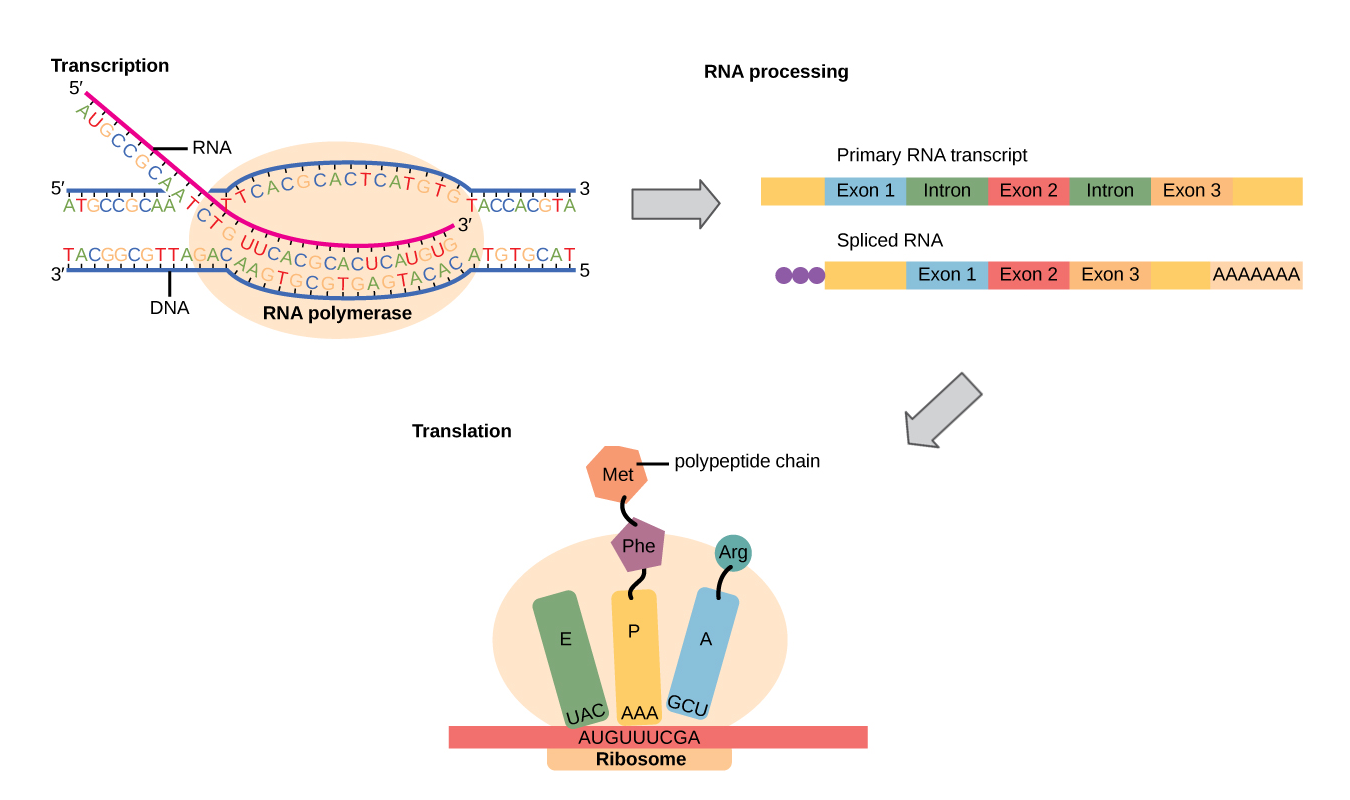
\includegraphics[width=\textwidth]{documents/latex/figures/1/dogma.png}
    \caption{Transferencia de la información genética. El ADN es transcripto en forma de ARN (ARN mensajero). Luego el ARN mensajero es ensamblado uniendo los exones (partes codificantes del gen) en un proceso denominado \textit{splicing}. Por último, los ribosomas usan la información del ARN mensajero para unir los aminoácidos en forma de proteína. Imagen tomada de OpenStax \cite{OpenStaxCNX}.}
    \label{fig:esquema_dogma}
\end{figure}

\begin{figure}[H]
\centering
    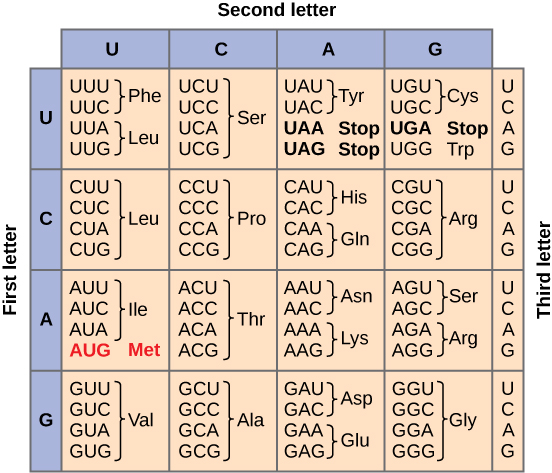
\includegraphics[scale=0.8]{documents/latex/figures/1/tableCodon.jpg}
    \caption{Tabla de codones para generar un determinado aminoácido o símbolo de terminación (\textit{Stop}). Imagen tomada de OpenStax \cite{OpenStaxCNX}.}
    \label{fig:table_codon}
\end{figure}

\newpage

\subsection{Variaciones genéticas}

Las variaciones genéticas son diferencias en el ADN entre individuos de una población \cite{EMBL}. Estas variaciones pueden ser causadas por mutaciones en el momento de la replicación del material genético, pudiendo ser de carácter permanente. Las mutaciones genéticas suelen representar un porcentaje muy pequeño con respecto a la secuencia completa del genoma (alrededor del 0.5\%), pero muchas de ellas suelen ser responsables de variaciones fenotípicas, es decir, nuestros rasgos ``observables''. 

Estas variaciones se pueden dividir en tres grupos principales:

\begin{itemize}
    \item Polimorfismos de un sólo nucleótido (SNPs): sustitución de un único par de bases. 
    \item Inserciones o deleciones (indels): pueden ocurrir en un intervalo grande del ADN de entre 2 a 200 pares de bases.
    
    \item Variaciones estructurales: ocurren en secuencias largas de bases, y pueden ser indels, inversiones, duplicaciones, entre otras.
    
\end{itemize}

Finalmente, cualquiera de estas variaciones pueden ser beneficiosas para el organismo, neutrales (sin efecto alguno) o perjudiciales. 

\subsection{Polimorfismos de un sólo nucleótido (SNPs)}

En el marco de esta tesis estudiaremos los polimorfismos de un sólo nucleótido, o SNPs por sus siglas en inglés (Single Nucleotide Polymorphism). Una persona posee en promedio alrededor de 4 a 5 millones de SNPs. Mientras la mayoría de ellos no tiene efecto en su desarrollo, algunos de ellos pueden variar la respuesta a ciertas drogas, o el riesgo de sufrir algunas enfermedades.

En la figura \ref{fig:snp_types} podemos ver los distintos tipos de SNP. De acuerdo al lugar, pueden ocurrir en una zona codificante, es decir una porción del gen que codifica una proteína, o en una zona no codificante, como los intrones (partes del gen no codificante).

Dentro de las sustituciones en la zona codificante, algunas mutaciones pueden ser sinónimas, es decir que existe un cambio en uno de los nucleótidos del ADN pero no genera un cambio en el aminoácido que codifica. Podemos ver en la tabla \ref{fig:table_codon} que muchos codones codifican el mismo aminoácido, por ejemplo, los codones AUU, AUC y AUA codifican el aminoácido isoleucina. Luego, si en la cadena de ADN, el codón AUA sufre una mutación en su último nucleótido, pasando a ser AUC, dicho codón seguirá codificando para el mismo aminoácido. Otro tipo de sustituciones, denominadas mutaciones sin sentido (\textit{nonsense}) codifican un codón de terminación (\textit{stop}), que resulta en un fin de codificación prematuro y en general una proteína no funcional.

En particular estudiaremos los SNPs con cambio de sentido (\textit{missense}), es decir aquellos que deriven en un cambio de aminoácido en la proteína producida por la variante del gen. 

\begin{figure}[H]
\centering
    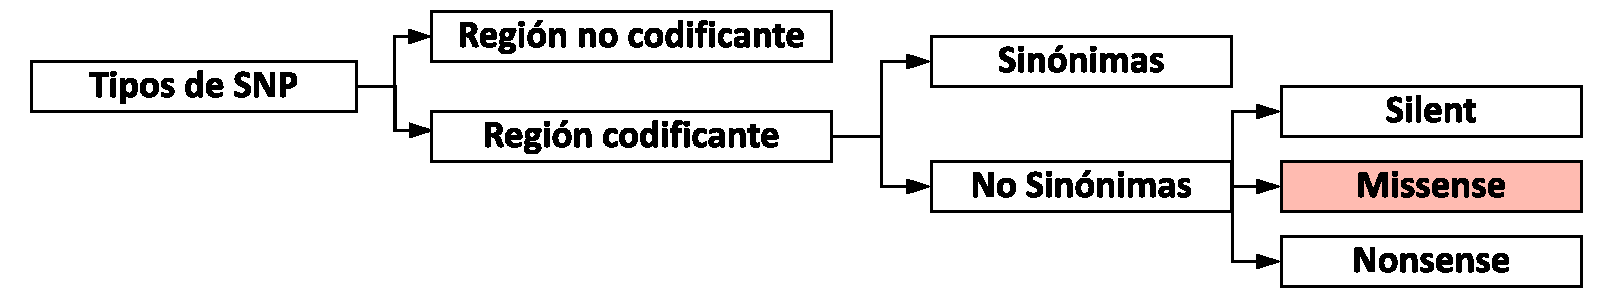
\includegraphics[scale=0.7]{documents/latex/figures/1/snp_types.pdf}
    \caption{Diferentes tipos de SNP de acuerdo a su posición en el genoma y su efecto. En este trabajo nos concentraremos únicamente en las sustituciones \textit{missense}. }
    \label{fig:snp_types}
\end{figure}

\subsection{Bases de datos ómicas}

En la actualidad existen diferentes bases de datos públicas (dbSNP, SNPedia, HapMap, entre otras) que registran millones de estos SNPs \textit{missense}. Los costos de una secuenciación completa siguen bajando de forma acelerada desde el Proyecto Genoma Humano \cite{sequencingcost} (ver figura \ref{fig:cost_per_genome}). Esto ha permitido generar un número creciente de estudios que permiten asociar polimorfismos genéticos a enfermedades (ver figura \ref{fig:dbsnp_growth_rate}). Diferentes bases, como Humsavar \cite{humsavar} o Clinvar \cite{clinvar}, contienen reportes curados con dichos resultados, que se actualizan periódicamente y pueden variar con nueva evidencia. Sin embargo, todavía existe un gran número de SNPs \textit{missense} de los cuales se desconoce su efecto en el organismo. 

% Side by side figures 
\begin{figure}[H]
\begin{minipage}[c]{0.45\linewidth}
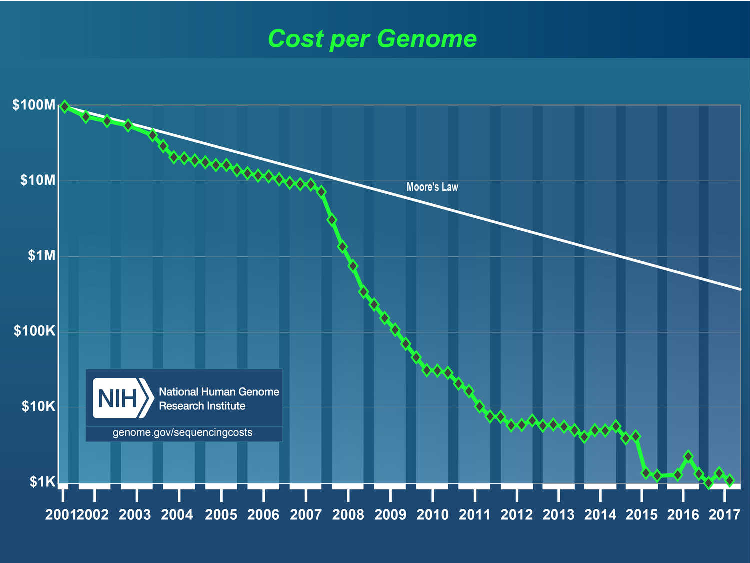
\includegraphics[width=\linewidth]{documents/latex/figures/1/costpergenome_2017.pdf}
\caption{Costo por secuenciación del genoma, NCBI-NIH, 2017. La curva verde corresponde al costo en dólares y la curva blanca equivale a la curva de la ley de Moore, es decir, si se reduciera a la mitad cada año.}
\label{fig:cost_per_genome}
\end{minipage}
\hfill
\begin{minipage}[c]{0.45\linewidth}
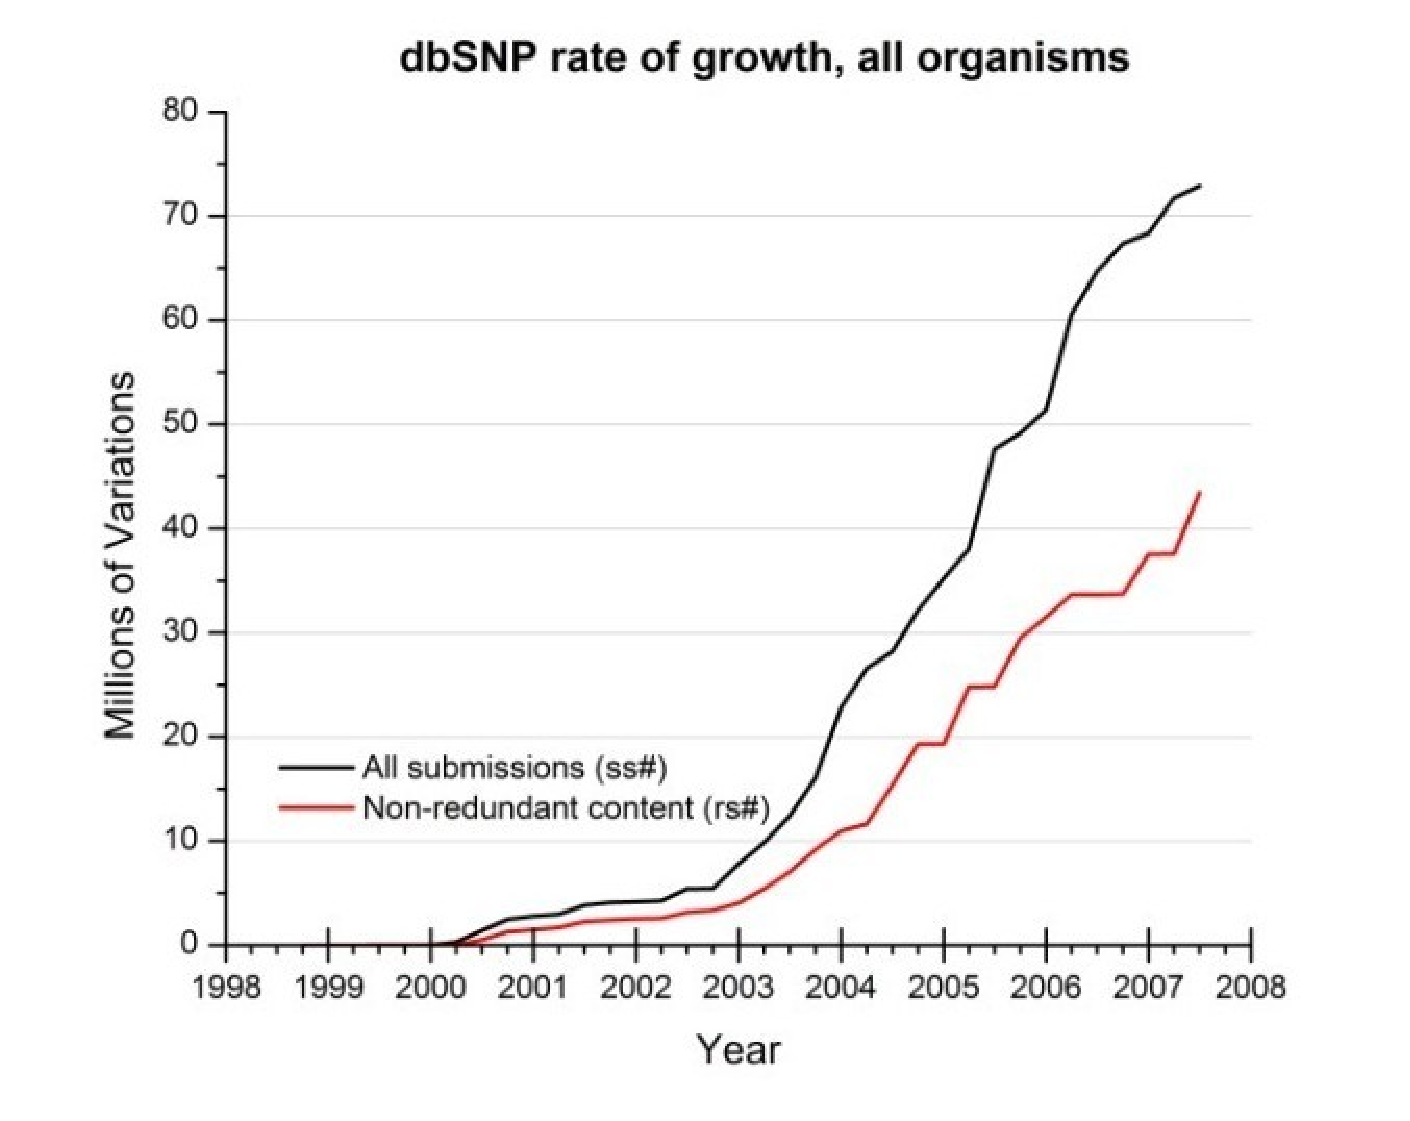
\includegraphics[width=\linewidth]{documents/latex/figures/1/increase_dbsnp.pdf}
\caption{Crecimiento de la base dbSNP a partir del Proyecto Genoma Humano, NCBI-NIH, 2008. La curva negra corresponde a todos los SNPs subidos a la base y la curva roja a los clusters de SNPs que referencian a la misma posición del genoma.}
\label{fig:dbsnp_growth_rate}
\end{minipage}%
\end{figure}

\textbf{El problema biológico que intentaremos atacar es poder predecir aquellos SNPs missense no investigados aún cuyo cambio en el aminoácido de la proteína generada pueda estar asociado a alguna patogénesis}. 

\section{Enfoque computacional}

Para abordar este problema, decidimos usar métodos de aprendizaje automático. El aprendizaje automático es un método computacional (dentro del área de la inteligencia artificial y la estadística) que consiste en aprender a partir de los datos. 

Existen diferentes formas de categorizar los algoritmos de aprendizaje automático. De acuerdo a Barber \cite{Barber2011}, una de las formas posibles es la categorización de acuerdo a la cantidad de tipo de supervisión durante la fase de entrenamiento. Este aprendizaje puede ser:

\begin{itemize}
\item Supervisado, en donde se utilizan ejemplos previos que están ``rotulados'', es decir que poseen una variable de respuesta conocida y se busca conseguir una predicción lo más certera posible sobre nuevos datos. Esta variable de respuesta puede ser continua (problema de regresión) o dividida en clases (problema de clasificación). 
\item No supervisado, donde el objetivo es encontrar distintos grupos o clusters dentro de los datos.
\item Semi-supervisado, en el que se trabaja con un pequeño conjunto de datos etiquetados y un conjunto mucho mayor de datos no etiquetados. El objetivo está en usar este último conjunto para mejorar el clasificador construido con los datos etiquetados.
\item Por refuerzo, donde un \textit{agente} observa el entorno y realiza diferentes acciones para maximizar la recompensa. El modelo a aprender entonces es la estrategia que le permite tomar decisiones ante determinadas situaciones. 
\end{itemize}

Durante la fase de entrenamiento estos algoritmos ajustan sus parámetros de acuerdo a los datos recibidos. En la mayoría de los casos estos algoritmos también poseen hiperparámetros, que no se modifican durante la fase de entrenamiento y determinan algunas de sus características. Estos hiperparámetros pueden ser optimizados mediante técnicas de validación cruzada (ver sección \ref{pipeline}). 

La creciente producción de trabajos nos aporta una gran cantidad de efectos conocidos de las variantes proteicas, y a su vez la ubicación (\textit{locus}) del SNP \textit{missense} responsable en el genoma. Estos datos se encuentran (en gran parte) de forma abierta y gratuita, lo que nos permite aplicar este enfoque computacional. Usando esta fuente de datos entrenaremos un modelo (de forma supervisada) que pueda predecir con un cierto grado de precisión el efecto de una variante aún no reportada. 

% \newpage

\subsection{Aprendizaje supervisado}

Como mencionamos anteriormente, el aprendizaje supervisado trata de predecir una respuesta usando un modelo generado con datos correctamente etiquetados. Definido de manera formal, dado un set de datos $ \mathcal{D} = \{(x^n, y^n), n = 1...N\}$  buscamos aprender la relación entre el ejemplo $x$ y la variable de respuesta $y$ tal que al recibir un nuevo ejemplo $x^*$ la respuesta predicha $y^*$ sea precisa \cite{Barber2011}. La precisión está definida formalmente por la función de pérdida o \textit{Loss Function}, $L(y^{pred}, y^{true})$. Esta función nos permite medir el costo de errar en la predicción y por lo tanto entrenar nuestro modelo de manera que el valor de la función de pérdida usando los datos de entrenamiento sea mínimo o cercano al mínimo.

En el contexto de nuestro problema, cada vector $x$ del set de datos $\mathcal{D}$ es un conjunto de variables que describen a distintos niveles (estructural, físico-químico, genómico) al SNP y a su variante proteica producida e $y$ es el efecto producido en el organismo, basándonos en reportes de Humsavar y Clinvar. Al ser una variable de tipo binaria, podemos aplicar algoritmos de clasificación para este problema.

A continuación haremos un recorrido por los distintos métodos de clasificación que utilizaremos en esta tesis. Estos métodos se encuentran implementados en el módulo \texttt{scikit-learn} de Python \cite{scikit-learn}, excepto por el método Gradient Boosting y su implementación XGBoost \cite{xgboost}. En cada uno de los apartados mencionaremos su funcionamiento general, sus parámetros y sus hiperparámetros. Para estos últimos mencionaremos entre paréntesis su nombre usado en la implementación.

\subsubsection{Regresión logística}

La regresión logística (LR) es un modelo basado en la regresión lineal. Al igual que ésta, consiste en buscar los coeficientes de una función de manera que el valor de la función de pérdida sea el mínimo. A diferencia de la regresión lineal, que usa una función lineal (o polinomial) para aproximar los puntos (que son valores continuos), la regresión logística usa la función logística para aproximar los valores (que son categóricos). Esta función, generalizada para múltiples variables predictoras y variable de respuesta binaria se define como:

\begin{equation*}
h_{\theta}(\boldsymbol{X}) = \frac{1}{1 + e^{\theta^{T}\boldsymbol{X}}} = Pr(Y = 1 | \boldsymbol{X}; \theta)
\end{equation*}

donde $\boldsymbol{X}$ representa el vector de variables predictoras, $\theta$ es el vector de coeficientes ($\theta^{T}$ representa al vector transpuesto) e $Y$ es la variable de respuesta \cite{Barber2011}. Lo que se busca modelar, es la probabilidad de pertenecer a una clase determinada (simbolizada con '1'), cuando las variables observadas son $\boldsymbol{X}$ y usando los parámetros $\theta$. La probabilidad de pertenecer a la otra clase entonces, es igual a 1 - $h_{\theta}(\boldsymbol{X})$. 

Los parámetros $\theta$ son obtenidos buscando maximizar la verosimilitud con los parámetros de la distribución real de los datos \cite{Hastie2001}, mientras que los hiperparámetros ($\Tilde{\theta}$) se obtienen usando validación cruzada (ver sección \ref{pipeline}). Los hiperparámetros que buscaremos optimizar son dos:

\begin{itemize}
    \item El parámetro de regularización (\texttt{C}): Parámetro usado para penalizar el uso de muchas variables en la función de pérdida, simplificando el modelo y previniendo un posible \textit{overfitting}.
    \item El balance de las clases (\texttt{class\_weight}): Pesos asociados a la importancia a la que se le da reconocer una determinada clase, penalizando el error en la función de pérdida con un valor asignado en lugar de 1. 
\end{itemize}

\subsubsection{Support Vector Machines}

Las Support Vector Machines (SVM) se desarrollaron inicialmente como métodos lineales de clasificación, al igual que la regresión logística. Esto significa que también buscan una frontera de decisión (\textit{decision boundary}) que define la clase a la que pertenecen los datos usando una combinación lineal de las variables predictoras. En este caso no se busca hallar los parámetros de la distribución a modelar sino que el objetivo reside en encontrar el hiperplano (\textit{Support Vector}) que mejor separe a los datos de entrenamiento \cite{Hastie2001}. Posteriormente este método fue extendido para buscar un hiperplano en un espacio de variables transformado (método no lineal). Esta transformación se logra reemplazando el producto interno por una función kernel. En este trabajo haremos uso de la función de base radial (RBF, por sus siglas en inglés), que es la más comúnmente usada en este método. En este algoritmo buscaremos optimizar dos hiperparámetros: 

\begin{itemize}
    \item El parámetro de penalidad (\texttt{C}): Este parámetro regula que tan bien debe el hiperplano separar las clases a costa de una distancia menor en la frontera de decisión. Es decir, un valor elevado de \texttt{C} se ajustará mejor a los datos de entrenamiento, mientras que un valor bajo será más general, a costa de errores.
    \item Gamma (\texttt{gamma}): Define que tan lejos alcanza la influencia de cada uno de los ejemplos de entrenamiento en la creación de la frontera de decisión.  
\end{itemize}  

\subsubsection{Random Forest}

A diferencia de los algoritmos anteriores, Random Forest (RF) esta basado en un método de clasificación basado en árboles de decisión. Estos métodos se caracterizan por segmentar el espacio de predicción en un número de regiones. Para entender Random Forest, resulta muy útil conocer el funcionamiento de éstos árboles. 

Un árbol de decisión se construye dividiendo el espacio de variables de forma recursiva, recorriendo la lista de variables y seleccionando la variable que mejor divide las clases de acuerdo a un criterio determinado. El criterio que decidimos usar en este trabajo, por ser el más usado en tareas de clasificación, es el índice Gini (también referido como pureza):

\begin{equation*}
    G = \sum_{k = 1}^{K} \hat{p}_{mk}(1 - \hat{p}_{mk})
\end{equation*}

donde $\hat{p}_{mk}$ representa la proporción de la clase $k$ en la región $m$ \cite{Hastie2001}. Uno de los principales problemas que presenta este enfoque es la alta varianza (\textit{variance}) con respecto a los datos de entrenamiento. Si la profundidad del árbol es muy grande, aumenta el riesgo de \textit{overfitting} en los datos que poseemos. 

En el caso de Random Forest, se construyen distintos árboles de decisión con subconjuntos de variables escogidos de forma aleatoria, con el objetivo de disminuir la varianza. A la vez, al ser árboles de poca profundidad (que favorecen el \textit{underfitting}), se genera una cantidad alta de árboles para solucionar el problema de alto sesgo (\textit{bias}). 

Esta técnica consistente en combinar distintos algoritmos para obtener un mejor predictor se la denomina \textit{ensamble}, y en particular, Random Forest se enmarca dentro de la técnica de \textit{bagging}. Esto significa que la predicción final se obtiene a través de un promedio de los predictores que componen el método con igual peso.

Una de las principales ventajas de Random Forest es su interpretabilidad. Esto se expresa en la posibilidad de calcular fácilmente la importancia de las variables en el modelo. La importancia de una variable (o \textit{feature importance}) se calcula como el promedio del índice Gini en cada uno de los nodos de los árboles donde aparece, expresada proporcionalmente a la importancia máxima de todas las variables \cite{Hastie2001}.
Finalmente, el algoritmos posee una serie de hiperparámetros a ser tuneados. Nosotros buscaremos optimizar los siguientes:

\begin{itemize}
    \item Profundidad del árbol (\texttt{max\_depth}): La profundidad máxima de cada árbol.
    \item Estimadores (\texttt{n\_estimators}): La cantidad de árboles.
    \item Cantidad de variables por árbol (\texttt{max\_features}): En cada split del árbol, se puede fijar la cantidad de variables a comparar.
\end{itemize}

\subsubsection{Gradient Boosting y XGBoost}

Gradient Boosting (GB) es otro método de ensamble, que como las otras técnicas de \textit{boosting}, genera modelos de forma iterativa, modificando el algoritmo para intentar corregir los errores de la iteración anterior. Esta es una diferencia crucial con respecto a los algoritmos de \textit{bagging}, como Random Forest, que genera modelos de forma paralela. La forma en que Gradient Boosting busca mejorar iterativamente es modelando el vector residual (o en otras palabras, la distancia entre la predicción y la variable a predecir) generando de esta manera un modelo aditivo que se puede representar de la siguiente manera:

\begin{equation*}
    F_{m}(X) = F_{m - 1}(X) + \eta \cdot \Delta_{m}(X) 
\end{equation*}

donde $F_{m - 1}(X)$ es el modelo del paso anterior, $\Delta_{m}(X)$ es el modelo del vector residual y $\eta$ es el \textit{learning rate}, un hiperparámetro que busca regularizar la importancia de este factor en el modelo final para reducir el \textit{overfitting} \cite{gradient}. 

En este trabajo vamos a utilizar XGBoost (XGB), una implementación de Gradient Boosting con árboles muy utilizado en competencias Kaggle \cite{xgboost}. Este algoritmo cuenta con una gran cantidad de hiperparámetros, al ser un método de ensamble combina los hiperparámetros de los \textit{tree boosters} con los pertenecientes al método Gradient Boosting. Decidimos limitarnos a un número relativamente pequeño de hiperparámetros buscando referencias de su uso, aunque dejamos la exploración de los restantes para un trabajo futuro. Los hiperparámetros explorados fueron:

\begin{itemize}
    \item Peso mínimo de las hojas (\texttt{min\_child\_weight}): Mínima suma del peso de las instancias (hessiano) necesaria en un hoja para dejar de realizar cortes.
    \item Gamma (\texttt{gamma}): Mínima pérdida requerida para la creación de un nuevo corte en el árbol.
    \item Muestreo (\texttt{subsample}): Proporción de muestra de los ejemplos antes de la construcción del árbol. 
    \item Cantidad de variables por árbol (\texttt{colsample\_bytree}): Mismo parámetro que en Random Forest.
    \item Profundidad máxima (\texttt{max\_depth}): Mismo parámetro que en Random Forest.
\end{itemize}

\subsection{Pipeline de entrenamiento, validación y evaluación} \label{pipeline}

Cada uno de estos métodos involucran una fase de entrenamiento, validación y evaluación. En la fase de entrenamiento los algoritmos ajustan sus datos de acuerdo a sus distintas funciones de pérdida. En nuestro trabajo también buscamos aproximarnos al mejor set de valores de hiperparámetros usando una técnica llamada \textit{Grid-Search}. Este método consiste en evaluar distintos valores para cada parámetro, que en conjunto forman una grilla (o \textit{grid}). 

Para cada conjunto de hiperparámetros de esta grilla se entrena el modelo y finalmente se elige el conjunto de hiperparámetros que haya tenido mejor performance (bajo alguna métrica, ver sección \ref{eval_metrics}). Al evaluar la performance de cada conjunto de hiperparámetros no podemos volver a usar el mismo conjunto de datos para el que fue entrenado, por lo que para evitar esto usamos otra técnica llamada \textit{k-fold Cross Validation}. La idea es generar un corte (\textit{split}) en el dataset de entrenamiento con el objetivo de poder evaluar los hiperparámetros en un conjunto de datos que no haya sido utilizado (conjunto de validación). Este procedimiento se realiza $k$ veces con diferentes splits realizados al azar, con una proporción igual en cada subconjunto o \textit{fold}. Una vez elegido el modelo entrenado con el mejor conjunto de hiperparámetros se evalúa en un dataset de evaluación (que no fue usado durante el entremiento) de acuerdo a las métricas de la sección \ref{eval_metrics}.

% \newpage

\subsection{Métricas de evaluación} \label{eval_metrics}

Las medidas que utilizaremos para evaluar la performance del modelo son las siguientes:

\begin{itemize}

    \item \textbf{Precisión}: La Precisión del modelo, está medida como la cantidad de positivos correctamente clasificados (VP) sobre la cantidad de instancias clasificadas como positivas: verdaderos positivos (VP) y falsos positivos (FP).
    
    \begin{equation*}
        \frac{VP}{VP + FP}
    \end{equation*}
    
% \pagebreak
    \item \textbf{Recall}: El Recall corresponde a la cantidad de verdaderos positivos sobre el total de positivos: verdaderos positivos (VP) y falsos negativos (FN).
    
    \begin{equation*}
        \frac{VP}{VP + FN}
    \end{equation*}
    
    \item \textbf{F1-Score}: El F1-Score es el promedio armónico entre la Precisión y el Recall. Usamos el promedio armónico de manera de afectar negativamente el resultado si alguno de los valores es especialmente bajo. Posee un rango de 0 a 1. 
    
    \begin{equation*}
        F_1 = \frac{2}{\tfrac{1}{\mathrm{recall}} + \tfrac{1}{\mathrm{precision}}} = 2 \cdot \frac{\mathrm{precision} \cdot \mathrm{recall}}{\mathrm{precision} + \mathrm{recall}}
    \end{equation*}
    
    % \newpage
    
    \item \textbf{Área bajo la curva ROC (AUC)}: La curva ROC está generada por dos métricas principales, FPR y TPR:
    
    \begin{multicols}{2}
        \begin{equation*}
        TPR = \frac{VP}{VP + FN}
        \end{equation*}
        \break
        \begin{equation*}
        FPR = \frac{FP}{FP + VN} 
        \end{equation*}
    \end{multicols}
    
    En un contexto de clasificación binaria, si ordenamos al score de predicción final de mayor a menor y consideramos positivos a todos aquellos a la izquierda del umbral de decisión (\textit{threshold}), obtendremos una tasa de verdaderos positivos y de falsos positivos (TPR y FPR respectivamente). Esto puede verse en la figura \ref{fig:threshold_auc}.
    
    \begin{figure}[H]
    \centering
        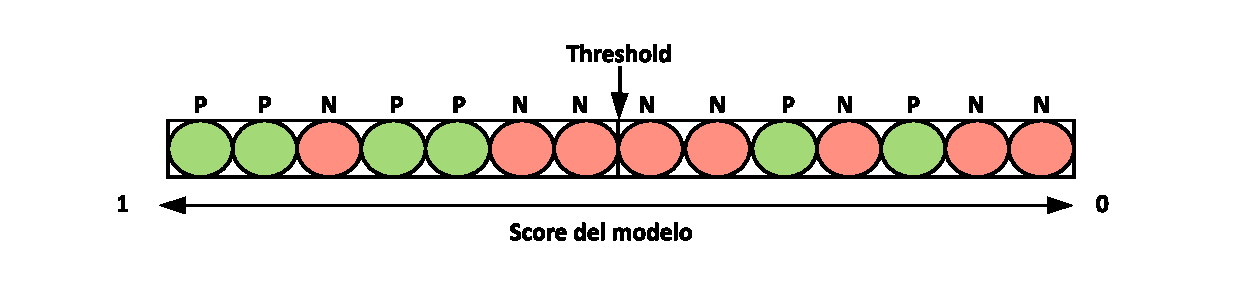
\includegraphics[scale=0.6]{documents/latex/figures/1/threshold_auc.pdf}
    \caption{Predicciones ordenadas de mayor a menor, donde el \textit{threshold} asigna clasificación positiva y negativa. El color de las instancias indica el valor real. En este caso el $TPR$ es igual a 2/3 y el FPR es igual a $3/8$.}
    \label{fig:threshold_auc}
    \end{figure}
    
    La curva característica operativa del receptor (ROC, por sus siglas en inglés) es la representación gráfica de la relación entre el FPR y el TPR al mover el umbral de decisión. 

    En la figura \ref{fig:example_roc} puede verse la curva que representa el ejemplo de la figura \ref{fig:threshold_auc}.
    
    \begin{figure}[H]
        \centering
        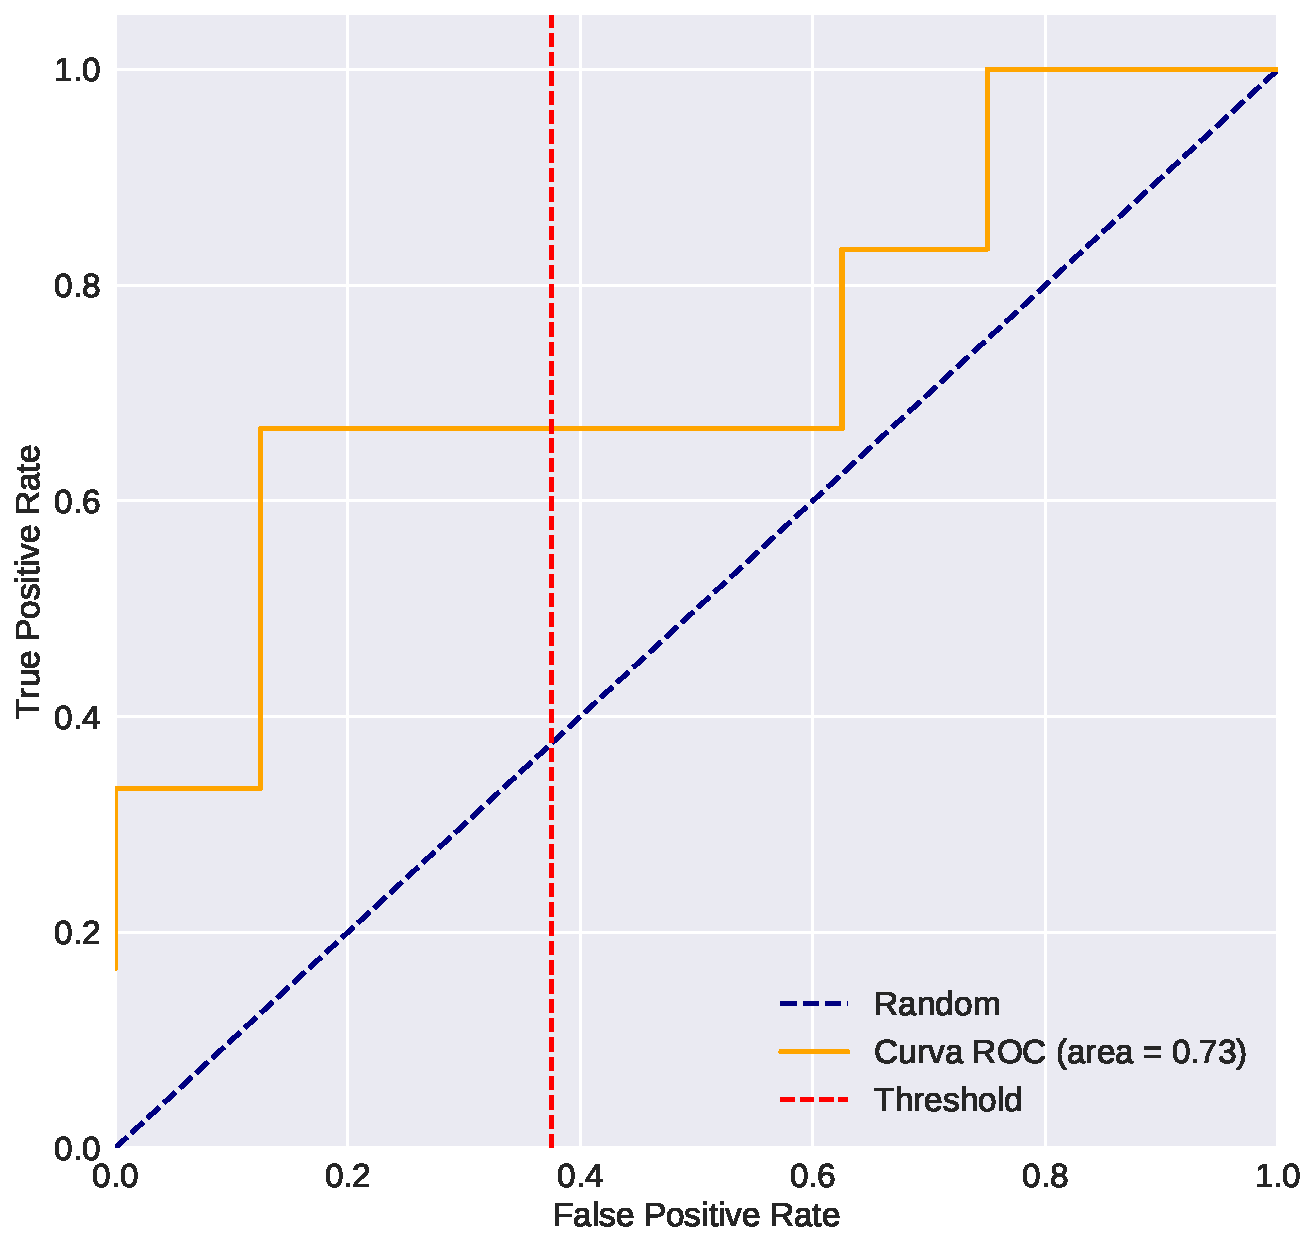
\includegraphics[scale=0.4]{documents/latex/figures/1/roc_ejemplo.pdf}
        \caption{Curva ROC de la clasificación de la figura \ref{fig:threshold_auc}. La línea punteada roja representa el umbral de decisión, que fijó el FPR y TPR en los valores anteriormente mencionados.}
        \label{fig:example_roc}
    \end{figure}
    
    Su área (AUC, por sus siglas en inglés) equivale a la probabilidad de que el modelo clasifique una instancia positiva cualquiera ``mejor'' que una instancia negativa cualquiera (estadístico Mann-Whitney $U$ \cite{doi:10.1256/003590002320603584}). Dadas dos muestras de tamaño $n_1$ y $n_2$, el estadístico Mann-Whitney $U$ se define como:
    
    \begin{equation*}
        U = \sum_{i = 1}^{n_1} r_{1i} - \frac{n_1 (n_1 + 1)}{2}
    \end{equation*}
    
    donde $r_{1i}$ es el ranking del elemento $i$ de la muestra $n_1$. La equivalencia con este estadístico viene de considerar a los verdaderos positivos y falsos positivos como muestras $n_1$ y $n_2$ respectivamente. Su distribución es aproximadamente normal para muestras grandes \cite{mann1947}, lo que nos permite calcular su intervalo de confianza. Otro método, el test de DeLong, utiliza este mismo concepto para evaluar y comparar curvas de AUC \cite{DeLong}.

\end{itemize}

% \newpage


\section{Trabajos relacionados}

A partir de mutaciones conocidas y sus propiedades asociadas, deseamos explorar un método de aprendizaje automático supervisado que nos permitan generar un modelo que, ante una mutación no estudiada, pueda predecir su patogenicidad. Para recolectar datos, asociados a mutaciones conocidas, existen múltiples herramientas. En particular, para el presente trabajo vamos a explorar: VarQ, VEST y FATHMM-MKL.

\subsubsection{VarQ}

VarQ es una herramienta generada en la BIA (Plataforma Bioinformática Argentina) por Leandro Radusky \cite{Radusky2017}. Esta herramienta permite extraer datos estructurales de variantes proteicas de un sólo aminoácido (SAS, por sus siglas en inglés) tomando información de diferentes bases de datos o aplicaciones (PDB, PFam, 3DID, entre otras), permitiendo el análisis manual de los diferentes cambios estructurales, como el tipo de actividad, el plegamiento, si pertenece a un sitio activo, o si forma parte en interfaces proteína-proteína, como se ve en la figura \ref{fig:varq_pipeline}. 

\begin{figure}[H]
    \centering
    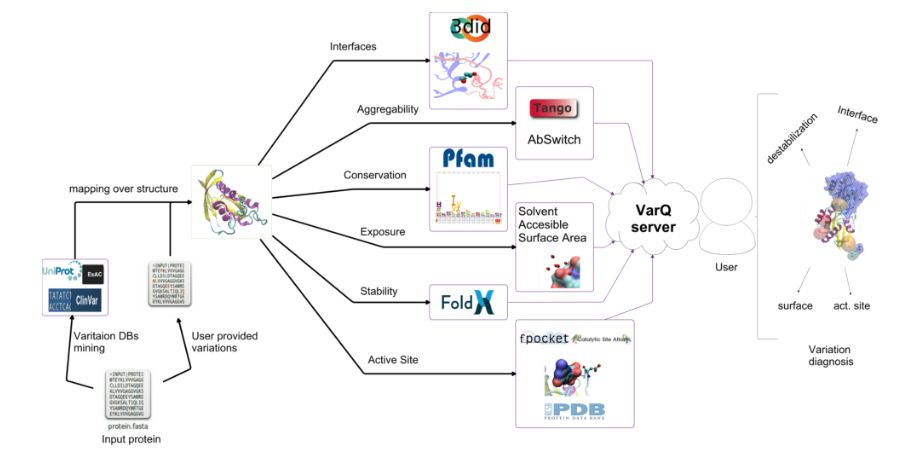
\includegraphics[scale=0.45]{documents/latex/figures/1/pipeline.png}
    \caption{Pipeline de extracción de datos de la herramienta VarQ. Esta figura fue extraída de la tesis de doctorado de Leandro Radusky \cite{Radusky2017}.}
    \label{fig:varq_pipeline}
\end{figure}

En la primera parte de esta tesis hacemos uso del trabajo de tesis de grado de Santiago Moreno (todavía en elaboración). Uno de sus objetivos principales fue generar un dataset de variantes a nivel de proteínas (al que denominaremos dataset VarQ), y evaluar la performance de un modelo que predice el efecto de la mutación usando las variables que provee esta herramienta. En la capítulo \ref{ch:desarrollo_varq} presentaremos un modelo de clasificación, variando las técnicas de aprendizaje automático presentadas, y creado en base a las variables que provee a este dataset. Posteriormente encontraremos sus limitaciones para tal fin.

\subsubsection{VEST}

VEST (\textit{Variant Effect Scoring Tool}) \cite{Carter2013} es un predictor de efectos funcionales de SNPs \textit{missense} desarrollado en el Karchin Lab de la Universidad de Johns Hopkins. Con esta herramienta (basada en Random Forest) analizaron aproximadamente 80,000 variantes anotadas de HGMD (\textit{Human Gene Mutation Database}) con variables de tipo genómicas, estructurales y físico-químicas usando la base de datos SNVBVox, desarrollado por el mismo equipo. A lo largo de nuestro trabajo integraremos muchas de las variables de esta base de datos a nuestros datasets.

\subsubsection{FATHMM-MKL}

FATHMM-MKL (\textit{Functional Analysis through Hidden Markov Models}) \cite{Shihab2015} es también un predictor de efectos funcionales de SNPs \textit{missense}, en regiones codificantes y no codificantes. El modelo está basado en SVM usando una combinación de múltiples kernels (\textit{Multiple Kernel Learning, MKL}). Fue desarrollado en la Universidad de Bristol. Uno de los puntos interestantes del trabajo es un suplemento con la descripción de las variables usadas. A partir de este informe buscaremos conseguir algunas de las variables usadas que hayan tenido mayor impacto en el modelo.

% \newpage


\section{Objetivos y estructura del trabajo}

El objetivo del trabajo se centra en responder una serie de interrogantes generados a partir del estudio de los trabajos previos:

\begin{itemize}
    \item El dataset de VarQ se compone esencialmente de variables de tipo estructural. ¿Es posible enriquecerlo con variables de otras dimensiones (físico-químicas, genómicas, filogenéticas)?
    \item ¿Cómo afectan las distintas variables a nuestros modelos de predicción de patogenicidad de los SNPs? ¿Cuáles son las más importantes para predecir una variante patogénica?
    \item ¿Cuáles son los mejores algoritmos de aprendizaje automático para resolver este tipo de problemas y cuáles son sus hiperparámetros?
    
\end{itemize}

Estos puntos serán abordados generando y estudiando modelos de aprendizaje automático sobre distintos conjuntos de variables descriptivas para los SNPs, como se describe a continuación:

\begin{itemize}
    \item Modelo usando el dataset VarQ
    \item Modelo usando propiedades físico-químicas de la proteína
    \item Modelo usando variables genómicas
    \item Integración de propiedades físico-químicas y variables genómicas
    \item Integración de propiedades físico-químicas, variables genómicas y las variables del dataset VarQ.
\end{itemize}




% \chapter{Materiales y Métodos}
% \label{ch:materiales}
% En esta sección detallaremos cada unos de los datasets usados durante nuestro trabajo, las distintas fuentes de atributos, y el esquema de clasificación usado.

\section{Análisis de los Datasets}

\subsection{Dataset VarQ}

El primer paso que tomamos fue realizar un análisis del dataset VarQ. Este dataset fue generado por la herramienta homónima generada en el BIA (Plataforma Bioinformática Argentina) por Leandro Radusky. Esta herramienta permite extraer datos estructurales de variantes proteicas de un sólo aminoácido (SAS, por sus siglas en inglés) tomando información de diferentes bases de datos o aplicaciones (PDB, PFam, 3DID, entre otras), permitiendo el análisis manual de los diferentes cambios estructurales, como el tipo de actividad, el plegamiento, si pertenece a un sitio activo, o si forma parte en interfaces proteína-proteína \cite{Radusky2017}. 

\begin{figure}[H]
    \centering
    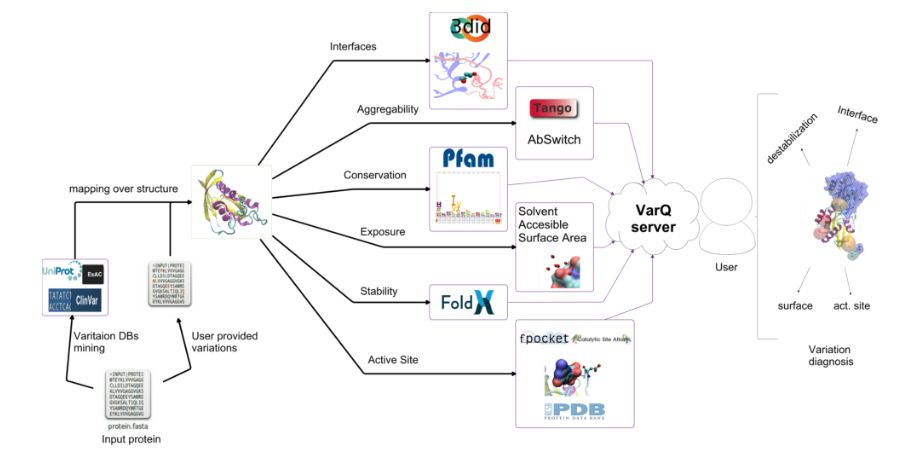
\includegraphics[scale=0.4]{documents/latex/figures/1/pipeline.png}
    \caption{Pipeline de extracción de datos de la herramienta VarQ. Esta figura fue extraída de la tesis de doctorado de Leandro Radusky.}
    \label{fig:varq_pipeline}
\end{figure}


Este dataset fue un acercamiento inicial al problema de predecir si a partir de una mutación en el gen. Para esto verificamos la calidad de cada una de las variables incluyendo el tipo. Validando el tipo de cada una de las variantes pudimos encontrar algunas de las que no se conoce a ciencia cierta su patogenicidad, por lo que fueron removidas. El dataset VarQ final tiene aproximadamente 17,8 mil variantes, de los cuales:

\begin{itemize}
    \item 11,7 mil están catalogados como benignos.
    \item 6,1 mil están catalogados como patogénicos.
\end{itemize}

Posee 12 columnas o variables: 

\begin{itemize}
    \item Mutant: Código identificatorio de la variante, compuesto por el código Uniprot, la posición del aminoácido donde ocurre la variación, y el cambio de aminoácido.
    \item SASA (Solvent-Accessible Surface Area): El área del aminoácido accesible por un solvente.
    \item SASA Percentage: El porcentaje del SASA sobre la superficie del aminoácido.
    \item B-FACTOR: Factor de temperatura correspondiente a un aminoácido en la proteína. Una mayor temperatura indica que el aminoácido pertenece a una zona potencialmente de mayor movilidad.
    \item Switchability: Factor de \textit{switching} del aminoácido \cite{Diaz2014}. Genera cambios en el plegamiento y por ende en la función de la proteína. 
    \item Aggregability: Usando el software Tango \cite{Fernandez-Escamilla2004}, evalúa la propensión del aminoácido a generar agregación desde un punto de vista estructural
    
\end{itemize}

\subsection{Humsavar}

Humsavar es una recopilación de SNPs anotados manualmente 


\section{Variables}

\subsection{ProtParam}

\subsection{VEST}

\subsection{SNVBox}


\section{Esquema de Clasificación}

\chapter{Desarrollo y Resultados}
\label{ch:desarrollo}
\section{Modelo usando el dataset VarQ}

Comenzamos nuestro trabajo analizando el dataset construido en la tesis de Santiago Moreno. Este dataset fue construido inicialmente con las variantes originales del sitio de VarQ, que consistieron en aproximadamente 400 mutaciones correspondientes a 13 proteínas con 10 variables. Posteriormente en el mismo trabajo se aumentó la cantidad para llegar a las aproximadamente 18 mil variables del dataset VarQ usando otras fuentes como Clinvar y Uniprot. Llamaremos a este dataset \textit{VarQ Completo}. 

\subsection{Limpieza del dataset VarQ Completo}

Para trabajar con este dataset decidimos verificar las etiquetas de cada una de las variantes, para confirmar que su status siguiera vigente. Así, cruzamos los datos con las fuentes originales usadas de Humsavar y Clinvar, y encontramos un subconjunto importante de proteínas que no aparecían en ninguna de las dos fuentes. Como puede observarse en la figura 3.1, de las 17.869 variantes del dataset, logramos encontrar 7.580 en la tabla de Clinvar, de los cuales sólo 2.397 tenían un estado confirmado como patogénicas, y 138 como benignas. El resto posee una caracterización difusa (por ejemplo, ``factor de riesgo''), y por lo tanto decidimos descartarlas. Cruzando el dataset con la tabla Humsavar encontramos una intersección de 7.261 variantes de los cuales 4.667 corresponden a patogénicas, 1.983 son benignas y el resto como ``no clasificado''. Decidimos mantener la clasificación de Humsavar en la intersección de los tres conjuntos. Esto nos deja con un dataset reducido de 7.418 variantes de las cuales 5.377 son patogénicas y 2.041 son benignas. Denominaremos a este dataset \textit{VarQ Reducido}. 

\subsection{Variables del dataset VarQ Reducido}

\begin{itemize}
    \item Variación de Energía (ENE): En \textit{VarQ}, las mutaciones son modeladas con el software FoldX, construye un modelo a partir de una estructura dada, mutando residuos específicos. El software predice el impacto energético de la mutación en la estabilidad de la proteína o, en caso de tratarse de un complejo, en la estabilidad del mismo.
     \item SASA : Es el valor correspondiente a la superficie accesible por parte del solvente, de la cadena lateral del aminoácido. Este valor permite determinar si la cadena lateral se encuentra en la superficie o en el núcleo de la estructura.
     \item Porcentaje de SASA: El porcentaje que representa el SASA sobre el total. Es decir el porcentaje que representa el SASA en función de la estructura de la proteína.
     \item B-Factor (BF): o factor de temperatura, que corresponde a un aminoácido dentro de la proteína. Una mayor temperatura, indica que el aminoácido pertenece a una zona potencialmente de mayor movilidad.
     \item Switchability (SWI): Evalúa cuán propenso a generar un cambio de hélice alfa a hoja beta es un conjunto de aminoácidos.
     \item Aggregability (AGG): El software Tango evalúa cuán
    propenso es un aminoácido a generar agregación en una proteína desde un punto de vista estructural. La agregación es el proceso por el cual proteínas mal formadas
    adoptan una conformación que causa su polimerización en fibrillas agregadas y organizadas. Muchas enfermedades neurodegenerativas (Amiloidosis) están asociadas con la agregación proteica.
     \item Conservación (CONS): Se calcula en bits, siempre y cuando la mutación pueda ser mapeada a una posición en una familia PFam asignada. Cuando una posición tiene un alto valor en bits y la
    misma posición coincide con el aminoácido conservado en la secuencia de la proteína
    interpretamos que dicha posición está altamente conservada. La misma puede estar
    altamente conservada porque es importante estructuralmente o porque es importante para
    la actividad enzimática. Los residuos con alta conservación tendrán un impacto mayor sobre la función pues afectan aminoácidos de la familia.
     \item Sitio Activo (AS): Las posiciones de sitio activo son
    aquellas que se encuentran marcados como unidos a ligandos en los archivos PDB o que
    pertenecen al mismo pocket que se encuentren conteniendo estos residuos nombrados o
    aquellos que pertenezcan al Catalytic Site Atlas.
     \item Interfaz 3DID: Determina si la posición sirve para una interfaz proteína-proteína según la base de datos de 3DID.
     \item Interfaz PDB: Determina si la posición sirve para una interfaz proteína-proteína según la base de datos de PDB.
\end{itemize}


\subsection{Descripción del dataset VarQ Reducido}

\subsection{Modelo creado a partir del dataset Reducido}

Si bien la cantidad de variantes patogénicas es mucho mayor que la cantidad de variantes benignas (es decir, el dataset se encuentra desbalanceado) decidimos generar un modelo para poder evaluar de forma superficial la dificultad del problema. Decidimos probar diferentes modelos (SVM, Regresión Logística y Random Forest) (\todo{Mostrar gráfico del rendimiento de cada modelo}), imputando la variables nulas con la mediana y estandarizando, y obtuvimos los mejores resultados en el caso del Random Forest. Cómo se puede observar en la figura 3.2 se obtuvo un AUC de 0,68. 

% Dado que la cantidad de variantes patogénicas en el dataset VarQ reducido es mucho mayor que la cantidad de variantes benignas decidimos generar 10 datasets distintos con las 2 mil variantes benignas y un subset aleatorio de 2 mil variantes patogénicas para obtener un conjunto de datasets balanceado de entrenamiento. Los resultados del algoritmo aplicado en cada uno de los datasets se promedió y se tuvo en cuenta la variación entre los resultados al momento de ser reportados. 
% En cada uno de los datasets se dividieron las variantes en subsets de entrenamiento (2/3 del total) y test (1/3 del total). Se entrenó con distintos algoritmos (Random Forest, Regresión Logística y Support Vector Machine), obteniendo el mejor resultado en el Random Forest. La curva AUC 

\begin{figure}[h]
    \centering
    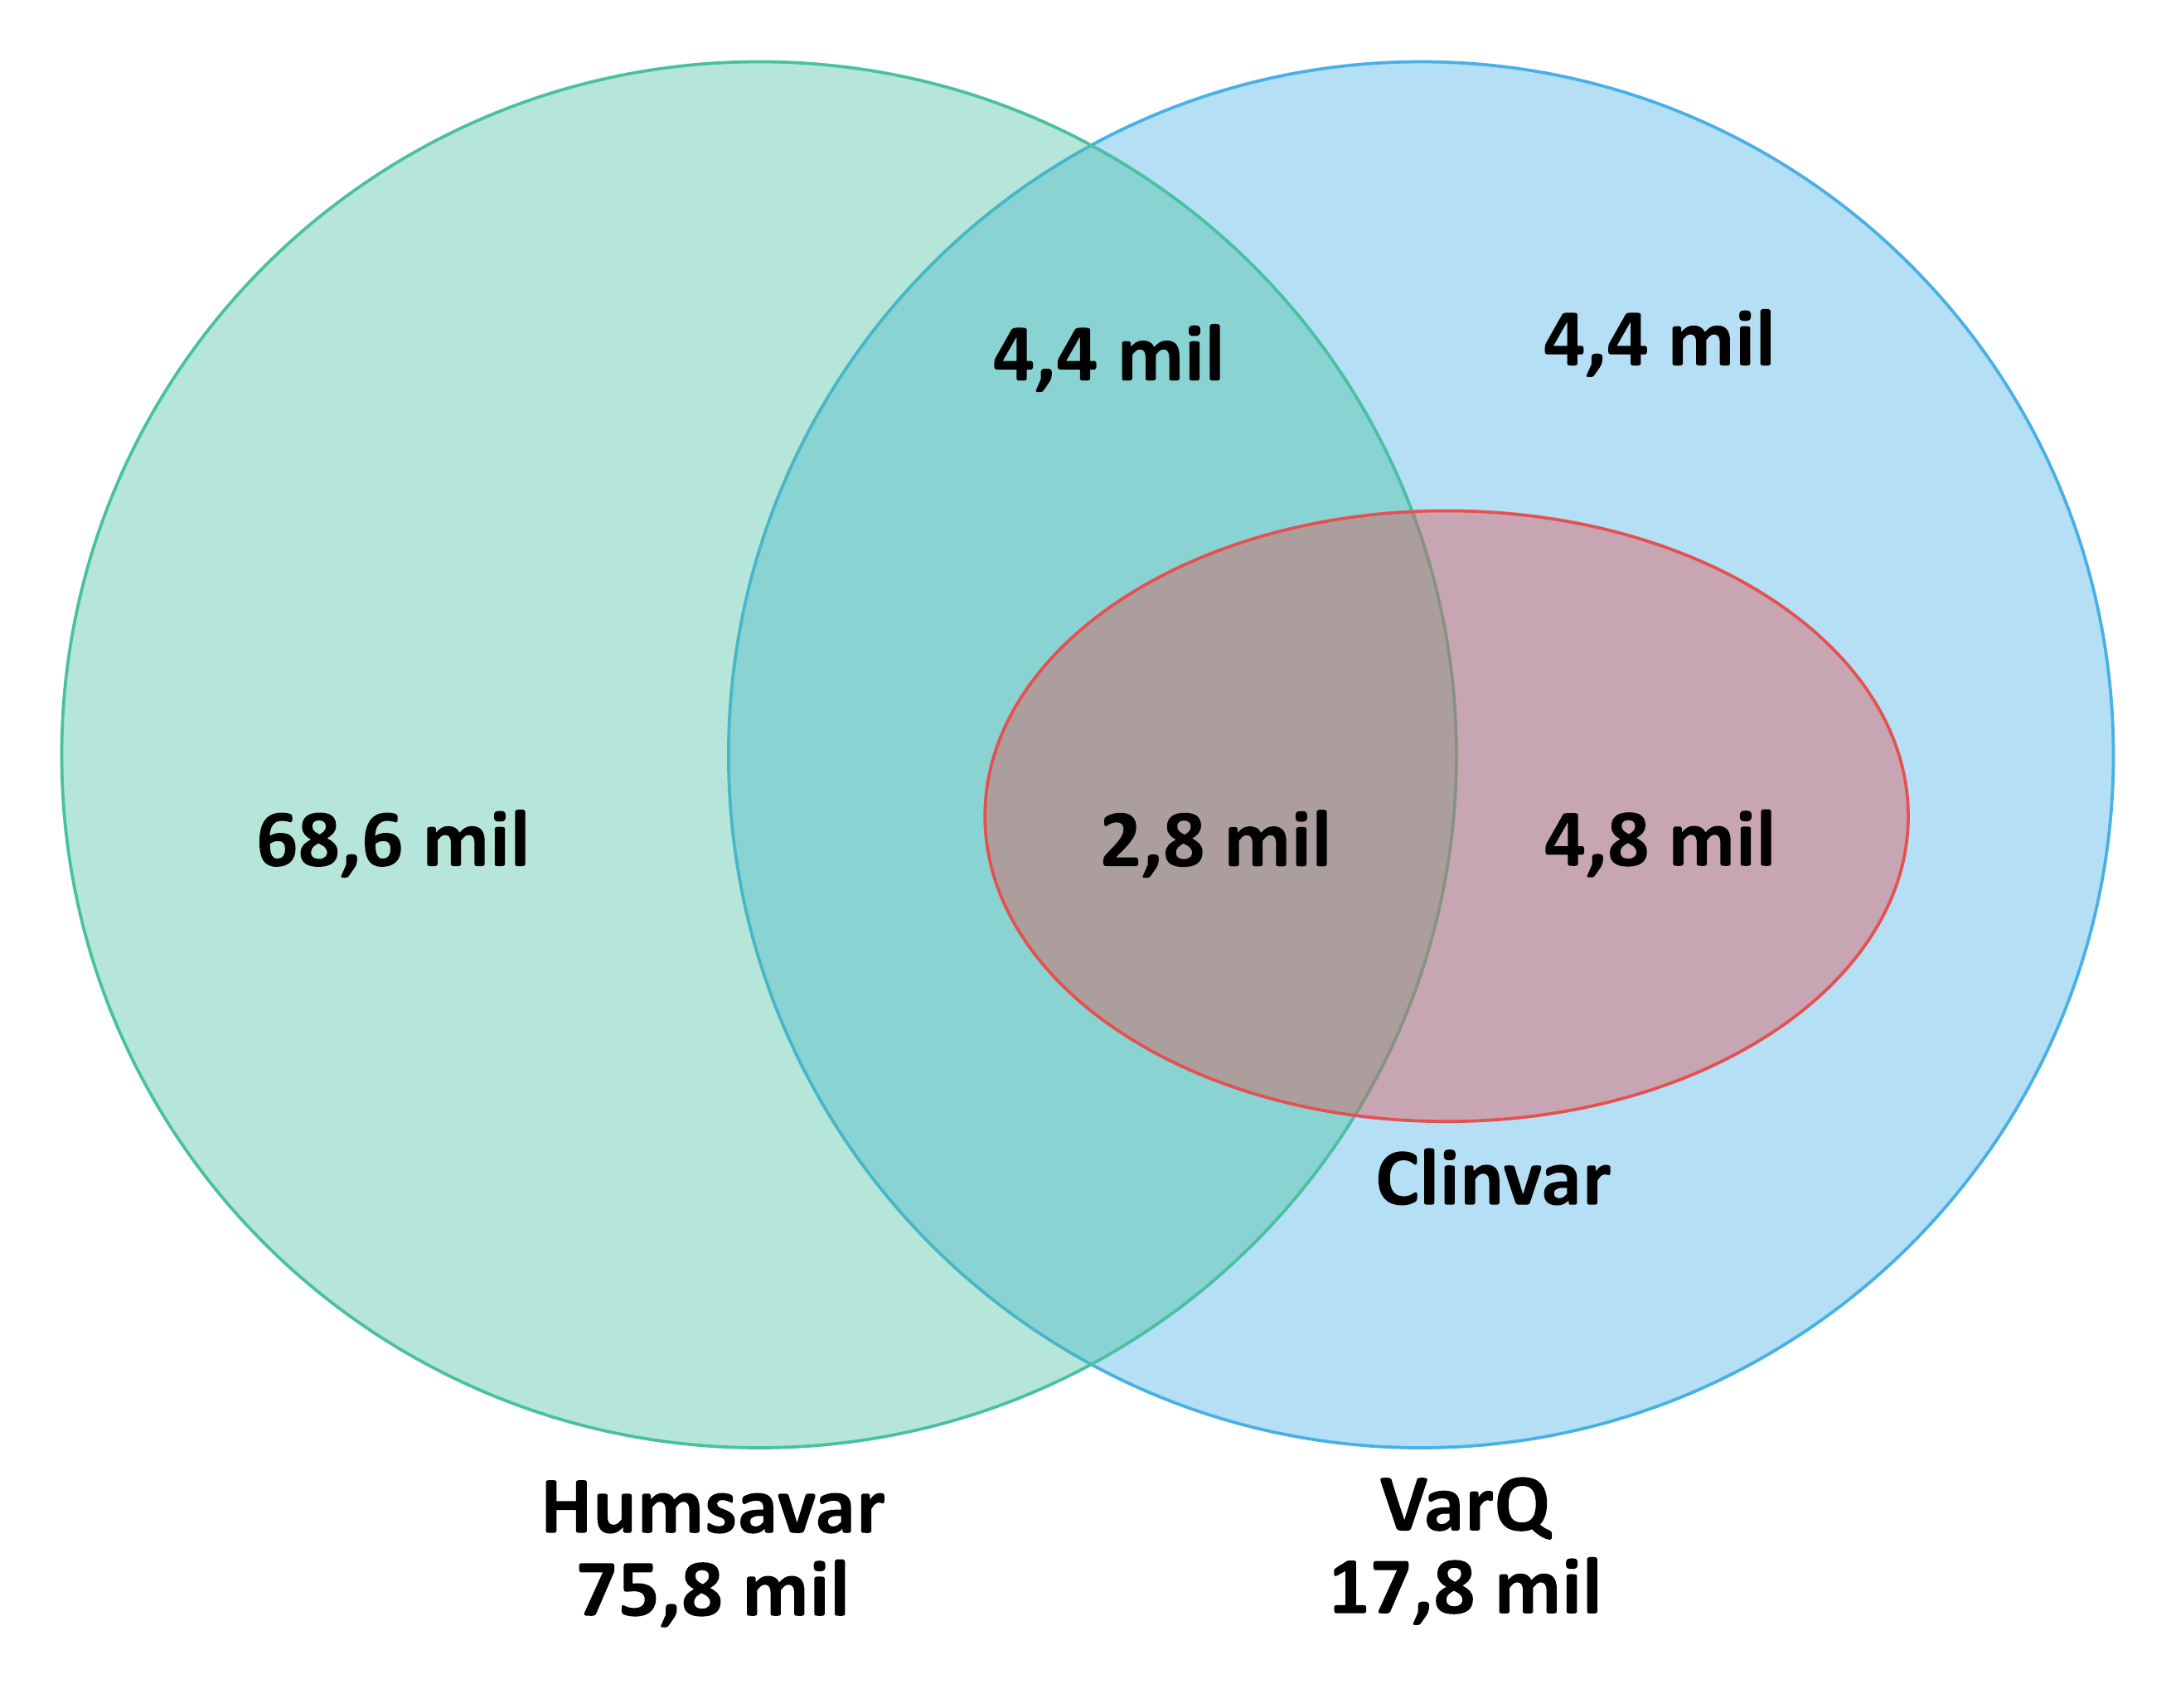
\includegraphics[scale=0.4]{documents/latex/figures/3/interseccion_varq.png}
    \caption{Valores en la intersección del dataset VarQ con las tablas Clinvar y Humsavar. \todo{Cambiar mil por k y dar números filtrando variantes sin etiquetas.}}
    \label{fig:interseccion_varq}
\end{figure}

\begin{table}[H]
\centering
\begin{tabular}{|l|l|l|l|}
\hline
              & Precisión & Recall & F1-score \\ \hline
Patogénicas   & 0.62      & 0.27   & 0.38     \\ \hline
Benignas      & 0.71      & 0.92   & 0.80     \\ \hline
Promedio      & 0.68      & 0.69   & 0.65     \\ \hline   
\end{tabular}
\caption{Reporte de métricas del modelo usando el dataset VarQ.}

\label{fig:metrics_varq}
\end{table}

\begin{figure}[h]
    \centering
    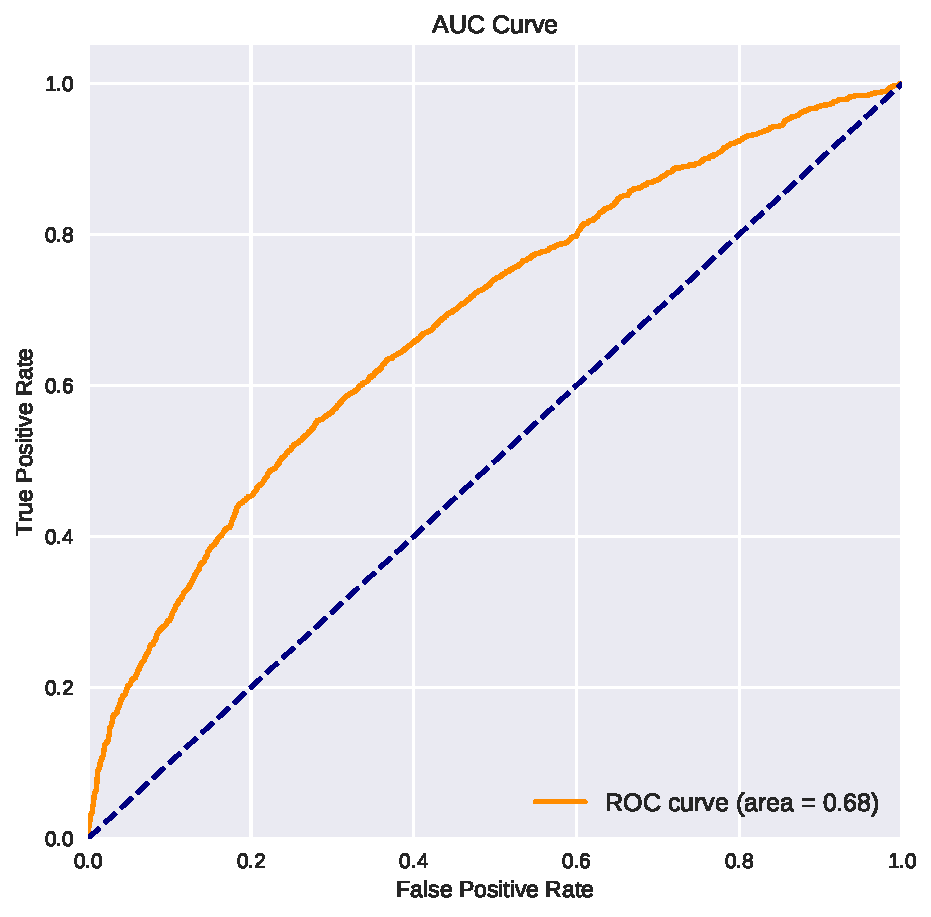
\includegraphics[scale=0.55]{documents/latex/figures/3/auc_varq.pdf}
    \caption{Curva AUC del algoritmo Random Forest del dataset VarQ. La línea punteada corresponde a un predictor Random. \todo{Correr para el nuevo dataset}}
    \label{fig:auc_varq}
\end{figure}

En la figura 3.3, la importancia de los features reportado por el algoritmo Random Forest puso en primer lugar con una gran diferencia a la variable que hace referencia al impacto energético de la mutación.  

\begin{figure}[H]
    \centering
    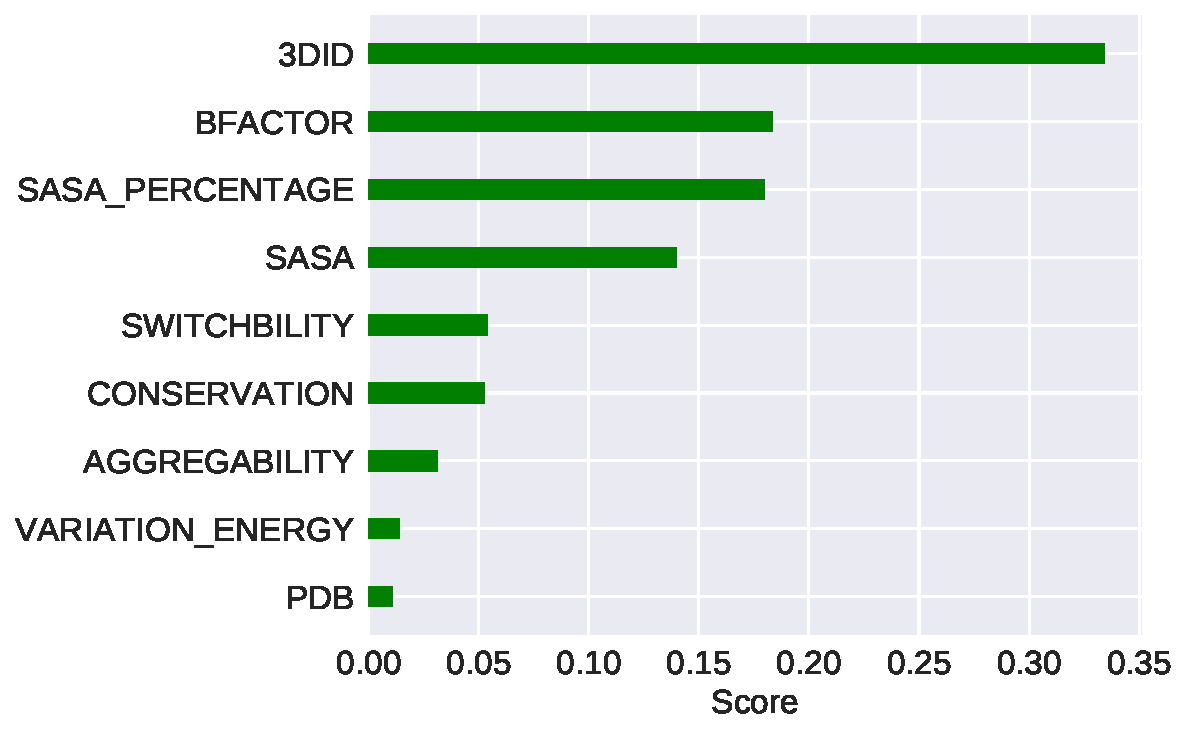
\includegraphics[scale=0.55]{documents/latex/figures/3/importances_varq.pdf}
    \caption{Los atributos más importantes del dataset VarQ usando un modelo Random Forest. \todo{Correr para el nuevo dataset}}
    \label{fig:importance_varq}
\end{figure}

\section{Modelo usando Propiedades Estructurales de la Proteína}

En esta sección generamos un nuevo dataset utilizando las variantes de Humsavar (a nivel de proteínas) buscando nuevas fuentes de información de carácter estructural de las proteínas.

Para el análisis de estas variable usamos el dataset de variables de Humsavar, que se compone de 68523 variantes (o ``mutantes'') de las cuales 39655 son variantes benignas (58\%) y 28868 (42\%) están asociadas a enfermedades. 

La primer fuente que utilizamos por su relativa facilidad en la extracción de un conjunto de variables físico químicas de la proteína fue el módulo ProtParam de la biblioteca Biopython. Esta biblioteca es un set de herramientas escritas en Python desarrollada por colaboradores para el área de la bioinformática, y posee una licencia de uso libre \todo{[citar]}.
El nombre ProtParam proviene de \textit{Protein Parameters} (parámetros de la proteína) y está basado en la herramienta del server proteómico Expasy \todo{[citar]}. Requiere el \textit{accession number} de la proteína (identificador único) o una subsecuencia de la misma para poder acceder a los parámetros calculados \todo{[citar]}, que son los siguientes:

\begin{itemize}
    \item Peso molecular
    \item pI Teórico
    \item Composición aminoácida
    \item Composición atómica
    \item Coeficiente de extinción
    \item Período de semi-desintegración o hemivida
    \item Índice de instabilidad
    \item Índice alipático
    \item Promedio de hidropaticidad
\end{itemize}

Para poder utilizar el módulo entonces recurrimos a Uniprot para conseguir el proteoma humano en formato FASTA. El formato FASTA fue desarrollado por David Lipman y William Pearson en 1985, y originalmente fue incluido en un programa del mismo nombre utilizado para el alineamiento múltiple de secuencias. Una archivo FASTA puede incluir diferentes secuencias, no necesariamente de aminoácidos, y cada una de estas secuencias posee una línea de descripción al comienzo que empieza con el símbolo $>$ \todo{[citar]}. Por ejemplo:

\begin{verbatim}
	>P01013 GENE X PROTEIN (OVALBUMIN-RELATED)
	QIKDLLVSSSTDLDTTLVLVNAIYFKGMWKTAFNAEDTREMPFHVTKQESKPVQMMCMNNSFNVATLPAE
	KMKILELPFASGDLSMLVLLPDEVSDLERIEKTINFEKLTEWTNPNTMEKRRVKVYLPQMKIEEKYNLTS
	VLMALGMTDLFIPSANLTGISSAESLKISQAVHGAFMELSEDGIEMAGSTGVIEDIKHSPESEQFRADHP
	FLFLIKHNPTNTIVYFGRYWSP
\end{verbatim}


A partir del proteoma obtenido se extrajeron las secuencias correspondientes a las proteínas del dataset Humsavar, y para cada una de ellas se tomó una subsecuencia de la misma alrededor de la posición donde se produjo la variante.

\vspace{2mm}
\todo{
TODO: Esquema de la subsecuencia
}
\vspace{2mm}

Para cada una de los parámetros calculados en ProtParam, generamos dos variables que buscan reflejar la diferencia generada por la variante. \todo{TODO: Hablar de los métodos usados}.
Además de la información obtenida vía ProtParam, recurrimos a una base de datos llamada SNVBox. Esta base de datos fue elaborada y es actualmente mantenida por el Karchin Lab de Universidad Johns Hopkins. Se encuentra en su versión 3.0 y sigue en desarrollo. \todo{Mencionar algunos papers que usaron esta base}. SNVBox posee alrededor de 90 variables consideradas relevantes para detectar el impacto biológico de un SNV \cite{Wong2011}, como datos sobre la estructura de la proteína, a nivel de aminoácido y también a nivel de los sitios de la proteína donde se encuentra la variante. Otra característica destacable de esta fuente es que posee dichas variables para todos los codones del exoma humano, lo que nos permitió una cobertura alta para las variantes del dataset con el que trabajamos.
Algunas de las variables encontradas fueron:

\vspace{2mm}
\todo{
TODO:
1. Lista de variables
2. Diagrama de SNVBOX
}
\vspace{2mm}

Luego del proceso del extracción de variables generamos un nuevo dataset cruzando estos atributos con las variantes de Humsavar. En el caso de los atributos relativos a los aminoácidos, pudimos cruzarlos usando la columna del dataset referente al identificador de la proteína, la posición de la variante, y el par de aminoácidos que se intercambiaron. Con los atributos relativos al genoma, pudimos cruzar la información usando la columna RSID (Reference SNP cluster ID). Esta columna identifica a un cluster de variaciones de un sólo nucleótido que pertenece a la misma posición en el genoma (o conjunto de posiciones) \cite{Ostell2007}. 
El dataset resultante (denominado dataset estructural) está compuesto por 68,5 mil variantes y 28 variables incluyendo la variable de respuesta (o tipo), de los cuales 39,6 mil son benignas (no se encontraron reportes de enfermedades en la literatura), y 28,8 mil variantes están asociadas a alguna enfermedad. 
Una de las formas que nos permite ver que tan bien las variables de este dataset están separando nuestros tipos de SNPs, es usar reducción de dimensionalidad. El primer método que probamos fue el análisis de componentes principales (PCA), con el que generamos dos componentes, que son combinaciones lineales de nuestras variables iniciales de forma de maximizar la varianza, es decir el par de componentes que mejor explican la información completa.

\todo{TODO: Poner gráfico de PCA}

Con este dataset generamos un modelo basado en un predictor Random Forest. Para la búsqueda de hiperparámetros usamos \textit{Grid-Search} (búsqueda ``en cuadrícula''). \todo{TODO: Evaluar RandomSearch}. Las variables se imputaron usando la mediana, y no fueron escalados al no ser necesario en algoritmos de clasificacion basados en árboles de decisión, dado que se evalúan las variables de forma independiente (\todo{cita?}). Se eligió inicialmente este tipo de predictor por ser el que obtuvo los mejores resultados en el dataset VarQ  con respecto a otros predictores (SVMs y Regresión Logística) y para centrar el análisis en cómo las variables afectan al modelo.  

Como puede observarse en la figura 3.4, a partir de este modelo se obtuvo un AUC de 0,71, que supera lo obtenido por el modelo usando el dataset VarQ. Las métricas observadas en la tabla 3.2 permiten dar cuenta de una precisión del 34\% con respecto a las variantes patogénicas, es decir, el modelo está reportando una 66\% cantidad de variables como patogénicas que no lo son (también conocido como error de tipo I), y un recall de 63\%, lo que indica que existe un 34\% de variables patogénicas en nuestro dataset que no están siendo detectadas por nuestro modelo (error de tipo II). \todo{TODO: Diagrama de errores}.

\begin{table}[H]
\centering
\begin{tabular}{|l|l|l|l|}
\hline
              & Precisión & Recall & F1-score \\ \hline
Patogénicas   & 0.34      & 0.63   & 0.44     \\ \hline
Benignas      & 0.88      & 0.67   & 0.76     \\ \hline
Promedio      & 0.76      & 0.67   & 0.70     \\ \hline
\end{tabular}
\caption{Métricas del modelo Random Forest aplicado al dataset estructural.}
\label{my-label}
\end{table}

% \subsection{Resultados}

\begin{figure}[h]
    \centering
    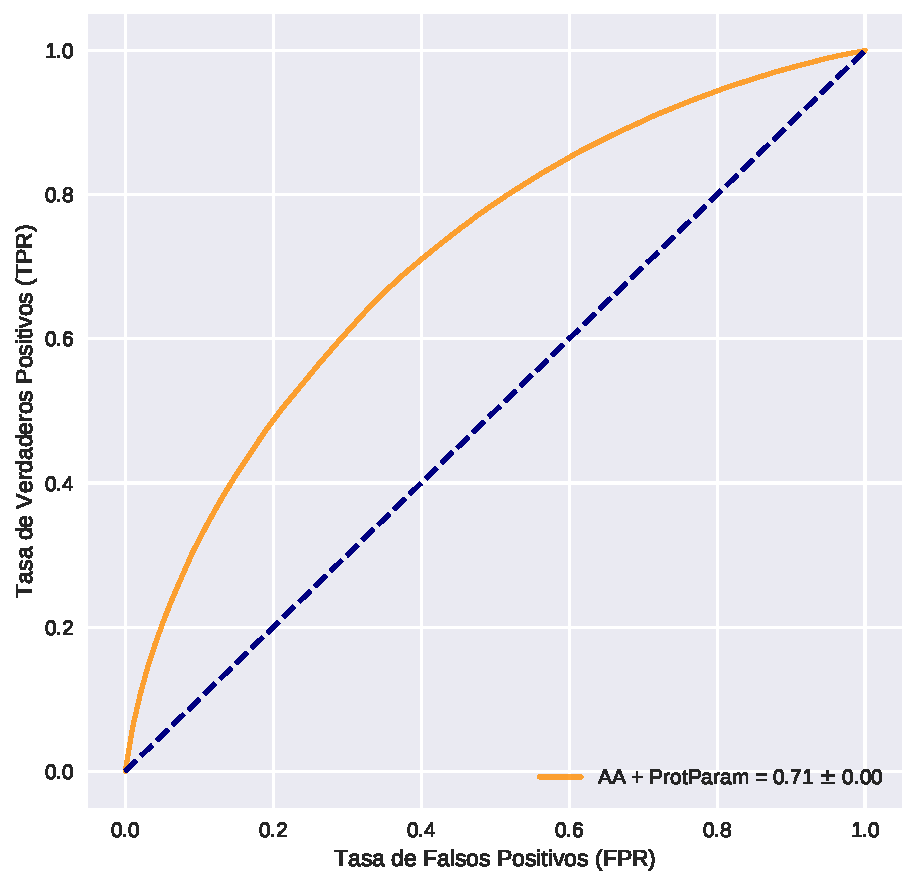
\includegraphics[scale=0.55]{documents/latex/figures/3/auc_1.pdf}
    \caption{Curva AUC del algoritmo Random Forest aplicado al dataset estructural. La línea punteada corresponde a un predictor Random.\todo{TODO: Correr modelo con un solo set train y test.}}
    \label{fig:auc_1}
\end{figure}

% \subsection{Importancia de los atributos}

El algoritmo nos permite identificar los mejores atributos dado su rango en cada uno de los árboles del clasificador. En este caso, podemos ver que los primeros tres atributos refieren a matrices de sustitución. Los siguientes features pertenecen a ProtParam, como la aromaticidad, la flexibilidad y la hidrofobicidad. La hidrofobicidad, o la capacidad de repeler el agua de la subsecuencia de los aminoácidos, es uno de las variables consideradas relevantes para definir la patogenicidad de una proteína, de acuerdo a \cite{Wang2016}. Por el otro lado, podemos observar variables con un nivel de importancia muy similar, como es el caso de PAM25, EX y BLOSUM. Estas variables corresponden a matrices de sustitución, y en la figura 3.6 podemos observar que existe una alta correlación entre ellas. \todo{TODO: Evaluar formas de variar el modelo usando variables que no esten correlacionadas. MRMR?} 

\begin{figure}[H]
    \centering
    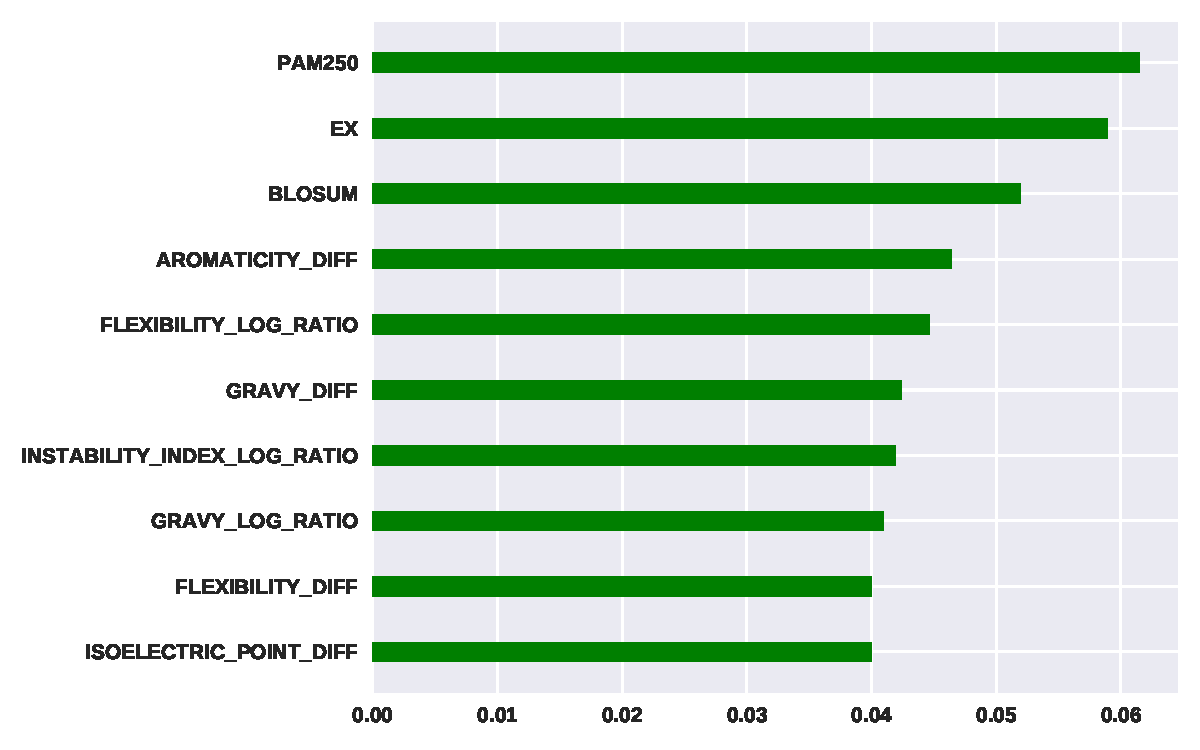
\includegraphics[scale=0.55]{documents/latex/figures/3/importance_1.pdf}
    \caption{Los 10 atributos más importantes del modelo Random Forest usando el dataset estructural. \todo{Falta eje x}}
    \label{fig:importance_1}
\end{figure}

% \subsection{Correlación}

\begin{figure}[H]
    \centering
    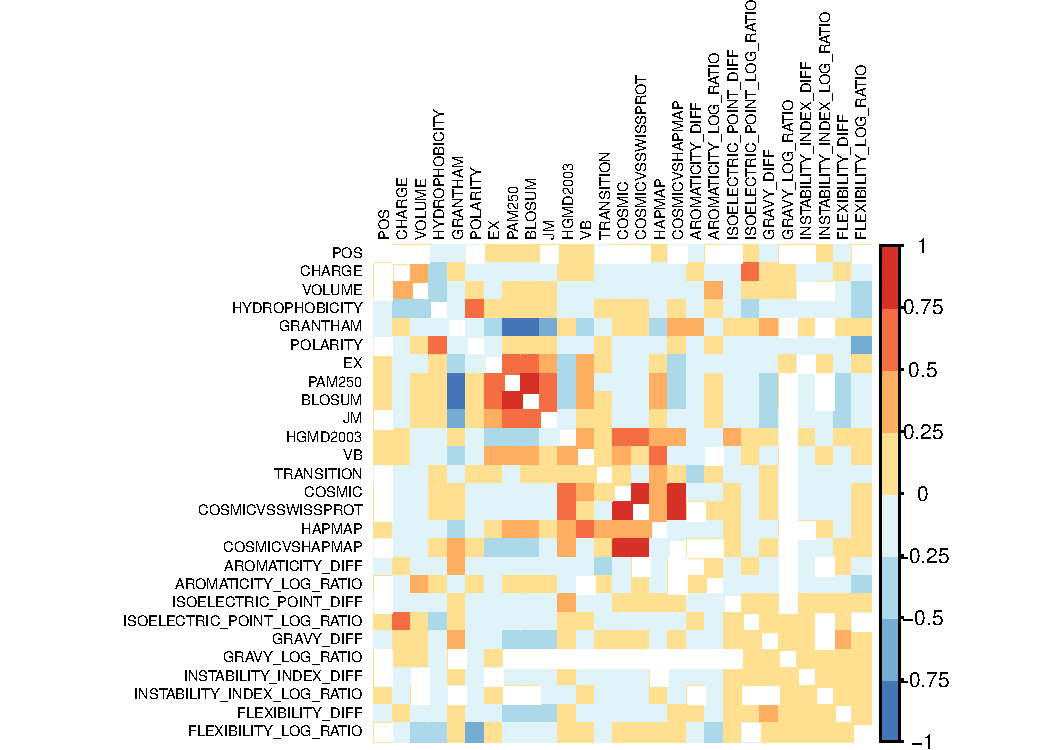
\includegraphics[scale=0.8]{documents/latex/figures/3/corrplot_1.pdf}
    \caption{Test de Correlación de Pearson (Significación: 0,05) sobre las variables del dataset estructural. Los valores en blanco poseen un p-valor por debajo del nivel de significación. Se puede observar que GRANTHAM se encuentra altamente anti-correlacionado con las matrices PAM y BLOSUM, mientras que estas se encuentran correlacionadas al igual que con EX.}
    \label{fig:corrplot_1}
\end{figure}

\section{Modelo usando Variables Genómicas}

Otra de las preguntas que nos hicimos al momento de comenzar este trabajo fue si las variables genómicas podían hacer un aporte al modelo, siendo que en los genes es donde se produce la mutación que finalmente da origen a la variante en la proteína. Como mencionamos preciamente, en la tabla Humsavar existe, para la mayoría de las mutaciones, el RSID o Reference SNP ID. Este identificador agrupa los distintos reportes que hagan referencia a la misma posición dentro del mismo genoma de referencia (hg19/GRCh37). A partir del RSID fue posible la consulta a la base de datos dbSNP (Versión snp150) con el que obtuvimos mayores detalles como ser el cromosoma, la posición y el cambio de nucleótido de la variante. 

En la literatura encontramos que dos de las variables genómicas asociadas a la conservación eran las que daban mejores resultados (modelos FATHMM-MKL \cite{Shihab2015} o VEST \cite{Carter2013}). Esta \textit{conservación} es un término biológico que refiere a las secuencias conservadas, es decir secuencias tanto genéticas como proteicas que se mantienen de forma similar o idéntica a en muchas especies que poseen un ancestro evolutivo en común (esta \textit{familia} de especies también se denomina árbol filogenético). En particular, la composición de estas variables consiste en alineamientos múltiples de secuencias genéticas (MSA) de 46 especies de vertebrados, incluyendo Homo Sapiens y otras como Felis catus (gato doméstico), Danio renus (pez cebra) y Equus Caballus (el caballo). En base a este alineamiento se usan dos medidas distintas de conservación, \textbf{PhastCons} \cite{siepel2005evolutionarily} y \textbf{PhyloP} \cite{Pollard2010}, que buscan detectar aquellas regiones en el genoma con mayor nivel de conservación entre las distintas especies. Decidimos incluir en nuestro dataset ambas medidas de conservación, usando el Table Browser de la Universidad de California, Santa Cruz \cite{Karolchik2004}.

También tomamos en consideración la función de la posición dentro del gen. La base de datos dbSNP define cada SNP de acuerdo a su clase funcional. Si la variación se encuentra cerca del intervalo de un transcripto, pero no en la región codificante, la clase funcional va a depender de la posición de la variación relativa a la estructura del transcripto \cite{Ostell2007}. Por otro lado, si la variación se encuentra en una zona codificante, la clase funcional se va a definir en base a si el alelo de la variación va a resultar en una sustitución sinónima (es decir, el nuevo codón va a formar el mismo aminoácido), una sustitución no sinónima (es decir, el nuevo codón va a formar un aminoácido distinto) o una sustitución sin sentido (en donde la mutación genera un codón de terminación prematuro).
Por último, usamos variables genómicas del dataset SNVBox, que calculan la conservación a 46 vías a nivel de exones, y la cantidad de SNPs conocidos en el exón donde se produjo la variante. \todo{TODO: Describir lista de variables del dataset}


A partir del dataset generado (llamado dataset genómico) podemos observar también como las variables permiten separar el dataset en dos clusters mucho mejor discriminados gracias a una combinación entre PCA y t-SNE.

\todo{TODO: Poner gráficos de PCA y t-SNE}

Luego de una primera aproximación al problema de encontrar las variables patogénicas generamos un modelo basado en Random Forest (volvimos a utilizar este algoritmo debido a los resultados obtenidos en el dataset VarQ y para facilitar la comparación entre datasets). En este caso volvimos a imputar las variables con su respectiva mediana.Por las razones descriptas en el capítulo anterior tampoco se escalaron las variables. Como se puede observar en la figura 3.7 obtuvimos un AUC de 0,89. 
Analizando la importancia de las variables (figura 3.8) en el modelo podemos observar que las variables de conservación están en los primeros dos puestos, confirmando lo obtenido por los trabajos de investigación antes mencionados. Por otro lado, esto genera un interrogante adicional: ¿Cuál es la razón por la que la variable \textit{Conservación} del dataset VarQ no genera un rendimiento similar?


\begin{figure}[H]
    \centering
    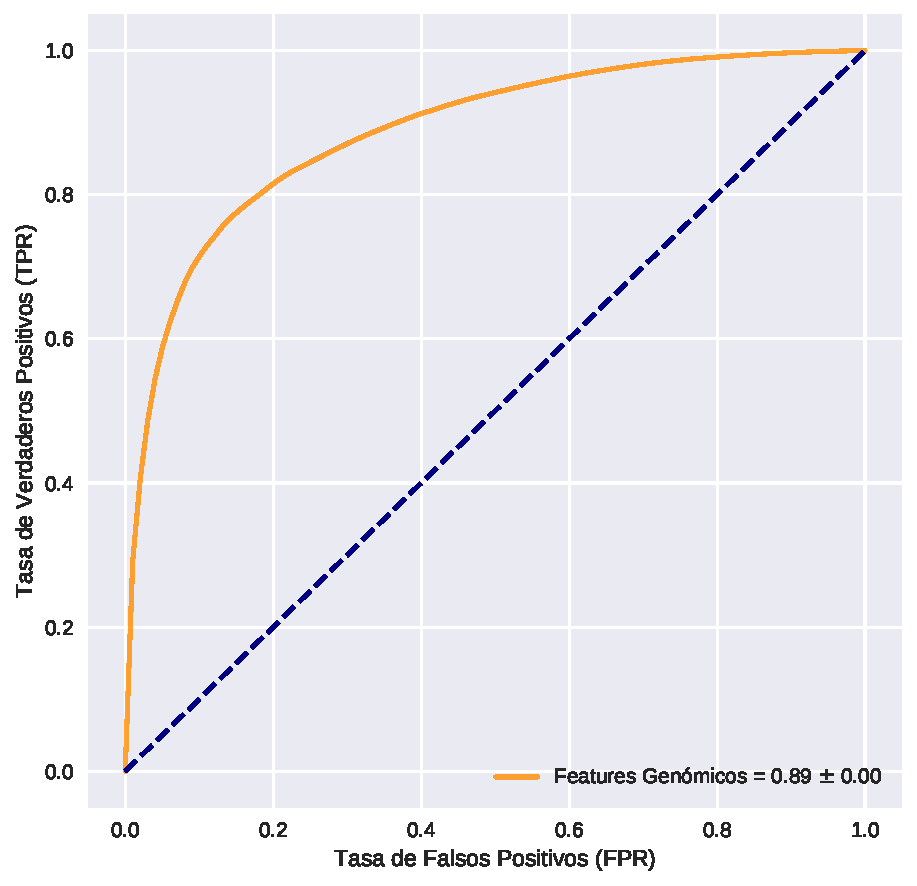
\includegraphics[scale=0.55]{documents/latex/figures/3/auc_2.pdf}
    \caption{Curva AUC del algoritmo Random Forest usando el dataset genómico. La línea punteada corresponde a un predictor Random.}
    \label{fig:auc_2}
\end{figure}

\begin{figure}[H]
    \centering
    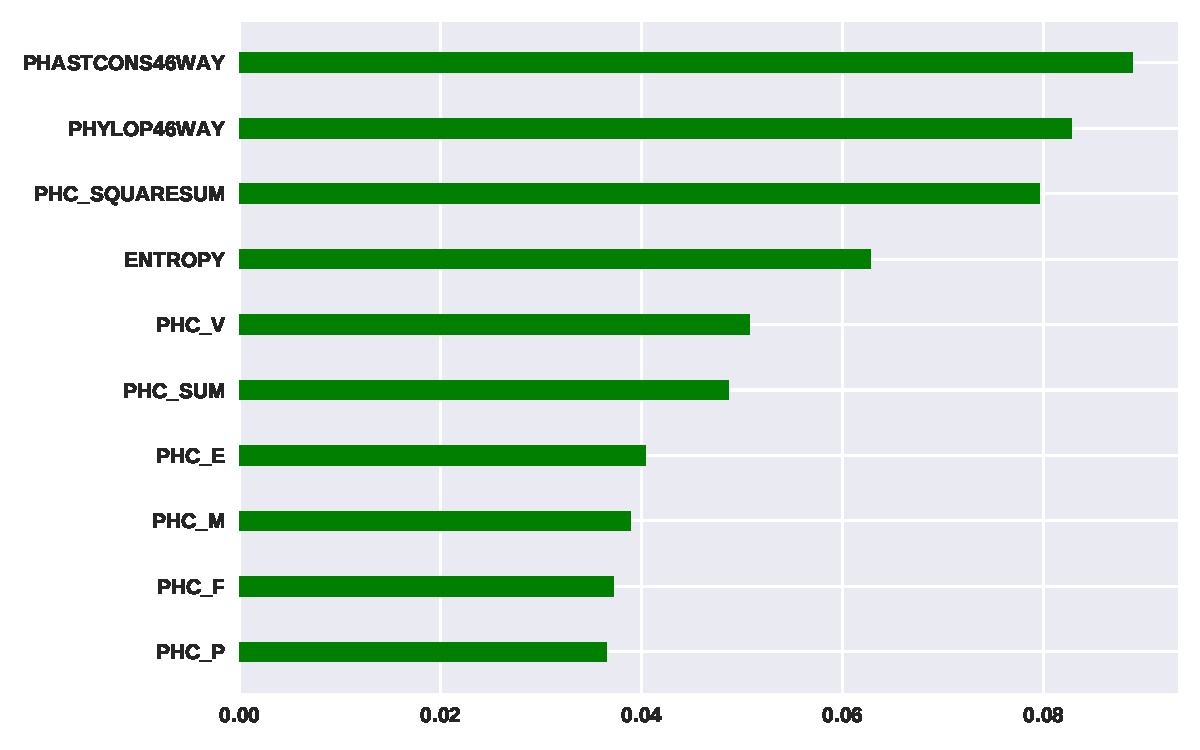
\includegraphics[scale=0.55]{documents/latex/figures/3/importance_2.pdf}
    \caption{Los 10 atributos más importantes del dataset genómico usando un modelo Random Forest. \todo{Falta eje X}}
    \label{fig:importance_2}
\end{figure}

Como podemos observar en la figura 3.8, el poder informativo de las variables de conservación es muy similar. La pregunta que nos hacemos en este caso es: ¿Las dos primeras variables de conservación están en los primeros dos lugares porque están altamente correlacionadas o aportan diferente información sobre las variables? La figura \todo{[x]} da una respuesta afirmativa a esta pregunta \todo{TODO: Hacer gráfico de correlación}. 

\todo{TODO: Gráfico de correlación y observaciones}

% \subsection{Descripción}
% \subsection{Correlación}
% \subsection{Resultados}

\section{Integrando el dataset estructural y el genómico}

Finalmente, unimos los dos conjuntos de variables para ver si representan una mejora frente a los ya excelentes resultados del modelo genómico. El modelo utilizado fue nuevamente Random Forest con imputación usando la mediana. Como se puede observar en la figura 3.9, no hubo una mejora significativa con respecto a los otros modelos. Las variables de conservación siguen encabezando la lista de las variables más importantes del modelo. Una posible hipótesis que explicaría estos resultados es que las variables del dataset genómico terminan ``eclipsando'' las del dataset estructural, y por lo tanto se pierde el subconjunto de variantes detectados por este último. Una forma de observar este efecto es cuantificar dichas variantes, es decir, ver si efectivamente el dataset estructural esta detectando una cantidad significativa de variantes no encontradas por el model genómico que no aparecen en este nuevo modelo. 

\begin{figure}[H]
    \centering
    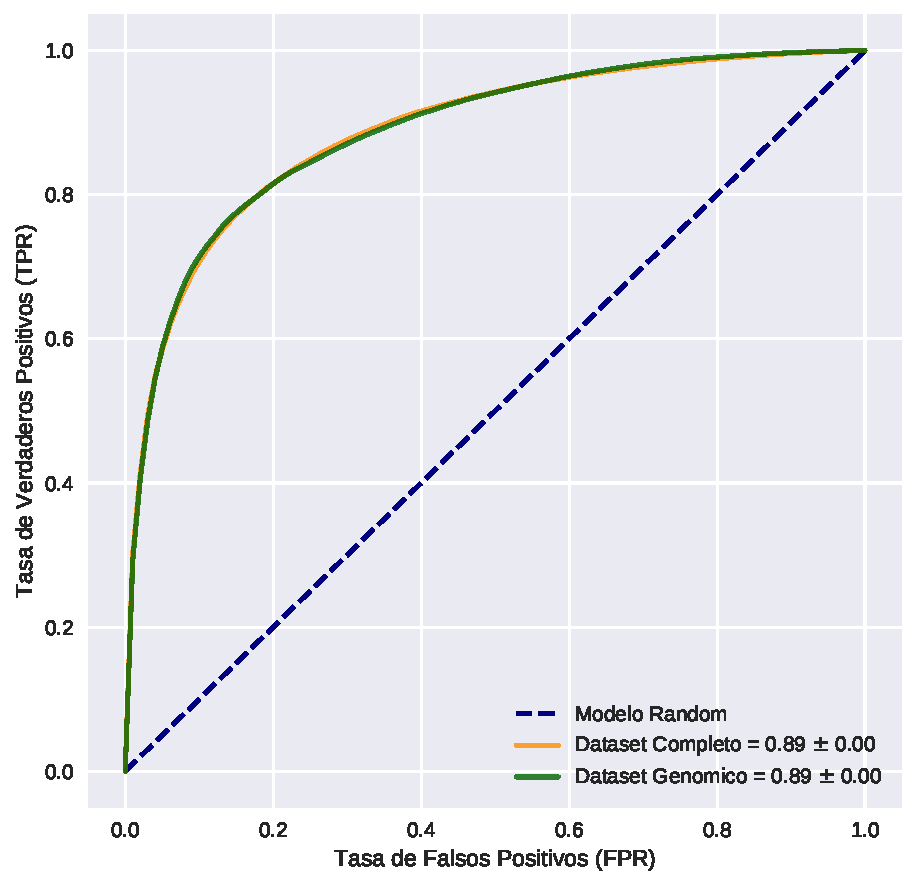
\includegraphics[scale=0.55]{documents/latex/figures/3/auc_3.pdf}
    \caption{Curva AUC del algoritmo Random Forest del dataset integral. La línea punteada corresponde a un predictor Random.}
    \label{fig:auc_3}
\end{figure}

\begin{figure}[H]
    \centering
    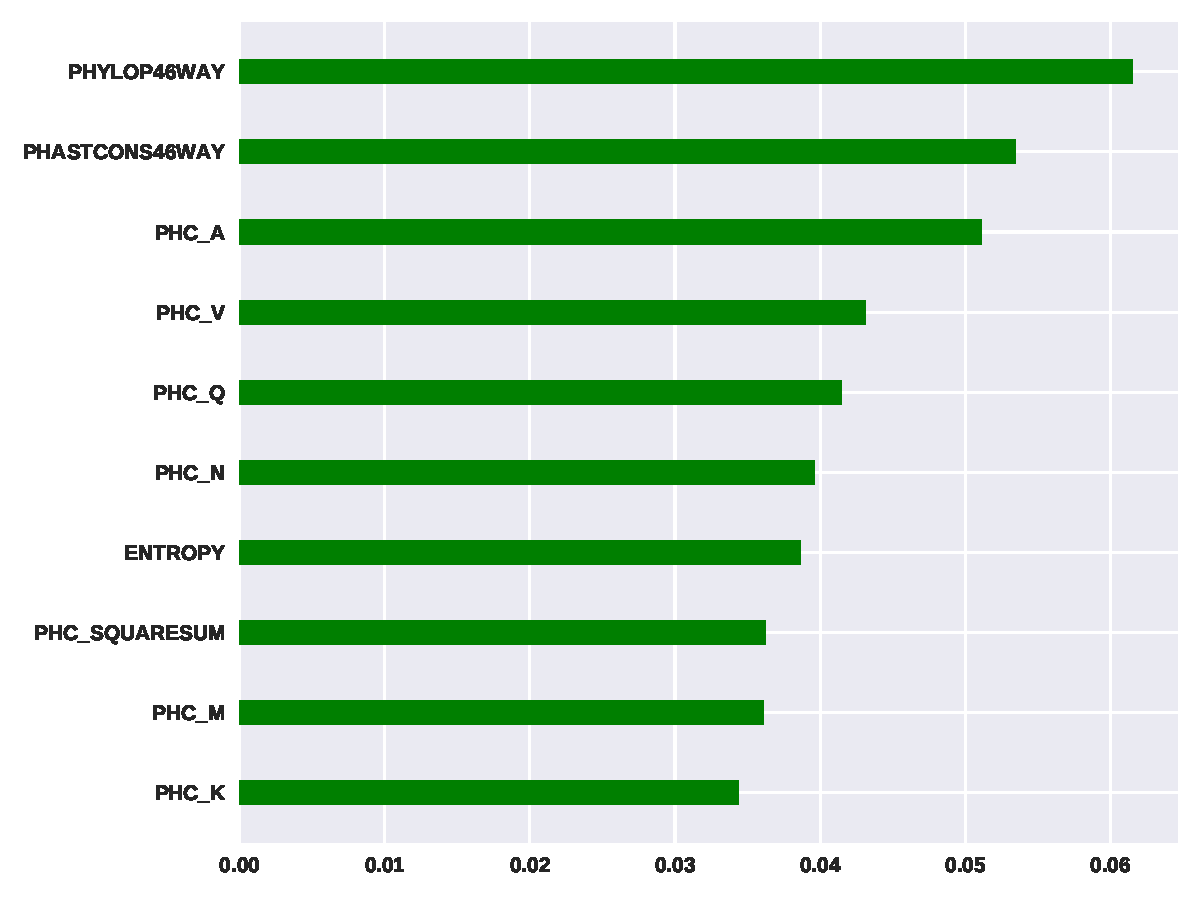
\includegraphics[scale=0.55]{documents/latex/figures/3/importance_3.pdf}
    \caption{Los 10 atributos más importantes del dataset integral.}
    \label{fig:importance_3}
\end{figure}
Una posible hipótesis que explicaría estos resultados es que las variables del dataset genómico terminan ``eclipsando'' las del dataset estructural, y por lo tanto se pierde el subconjunto de variantes detectados por este último. Una forma de observar este efecto es cuantificar dichas variantes, es decir, ver si efectivamente el dataset estructural esta detectando una cantidad significativa de variantes no encontradas por el model genómico que no aparecen en este nuevo modelo.  Ante esta situación una posible solución es usar algún método de ensamble que consiga potenciar al mejor de los dos modelos agregando las demás. Decidimos probar una serie de métodos clásicos de ensambling: Stacking, Bagging, y Boosting.

\todo{TO DO: Explicar métodos y exponer resultados.}
\todo{TO DO: Listar diferencias entre las variantes correctamente detectadas de los dos modelos.}
\todo{TO DO: Cambiar gráficos de AUC, cambiar train-test a uno solo. }

\todo{TO DO: Modificar diccionario de hiperparámetros del RF. Probar brevemente otros métodos para descartar que alguno sea muy superior.}

% \section{Uniendo las variables al Dataset VarQ}

% La siguiente pregunta es si el modelo mejora aún más sumando las variables de VarQ al conjunto de variables con los que trabajamos.




% \chapter{Conclusiones y Trabajo Futuro}
% \label{ch:conclusiones}
% En el presente trabajo mejoramos el modelo original pasando de un AUC de 0.74 a 0.90. Pero además hemos explorado diferentes aristas relativas al problema de predicción planteado con el objetivo de responder nuestros interrogantes iniciales. 

La primera pregunta era acerca de la posibilidad de enriquecer el dataset VarQ con nuevas fuentes de datos. Esta pregunta fue respondida afirmativamente, dado que agregar nuevas dimensiones demostró ser efectivo en la mejora del modelo, manteniendo fijo el algoritmo utilizado, siendo este Random Forest en todos los casos. En particular, el modelo que usó variables genómicas, arrojó un AUC de 0.85. El otro conjunto de variables analizado, las Físico-Químicas alcanzaron un AUC de 0.72. Si bien el AUC no fue superior al del modelo VarQ Curado, este demostró ser de utilidad. El modelo Integral, que combinó ambos datasets, resultó ser mejor que los dos anteriores, llegando a un AUC de 0.88 (figura \ref{fig:curvas_auc_humsavar}). Por último, sumar estas variables al dataset VarQ Curado también mostró una mejora, pasando de un AUC de 0.74 a 0.86 (figura \ref{fig:curvas_auc_varq}). 

La segunda pregunta que nos hicimos al comienzo del trabajo era sobre cómo la las variables afectan a nuestros modelos. La descripción estadística del dataset nos permitió entender como el método estándar para calcular importancia de variables en métodos de ensamble se ve afectado en variables altamente correlacionadas. Con respecto a las variables utilizadas, detectamos que las variables de conservación (phastCons y phyloP) son las más relevantes para nuestro problema de predicción. Si bien el dataset VarQ ya poseía variables de conservación, estas pertenecen a familias de proteínas (Pfam). Otras variables de importancia considerable son la variación de la energía (del dataset VarQ, obtenida vía PDB) y las matrices de sustitución o distancia (GRANTHAM, PAM250, BLOSUM, EX, JM y VB). Un aspecto destacable es que esta lista de variables corresponden a datasets distintos, reforzando la conclusión sobre la importancia de sumar dimensiones al problema.

Este trabajo también consistió en una comparación de distintos métodos de aprendizaje automático. En la primera sección del desarrollo comparamos tres métodos clásicos con el dataset VarQ Curado: Regresión Logística, Support Vector Classifier y Random Forest, obteniendo mejores resultados con éste último. Luego en la última sección del trabajo comparamos Random Forest con un método más avanzado de ensamble, XGBoost en los datasets Integral, mejorando la performance del modelo de un AUC de 0.88 a 0.90; y VarQ+Integral, llevando el AUC de 0.86 a 0.88.

\section{Trabajo Futuro}

Uno de los principales productos de este trabajo es la generación de un nuevo dataset que contiene numerosas variables estructurales y físico-químicos de la proteína, sumados a variables de tipo genómico. Este dataset también contiene variantes que están ligados a diferentes genes, que a su vez poseen cantidades distintas de SNPs potencialmente dañinos. Una de los trabajos que quedaron pendientes consisten en generar modelos individuales para cada gen, dado que puede existir un sesgo en nuestro modelo en caso de tener un número muy grande de SNPs de un gen determinado. También creemos que los trabajos futuros que deriven de este deberían hacer énfasis en la generación de modelos que mejoren la selección de hiperparámetros (en particular sugerimos el uso de técnicas de optimización bayesiana), y un tratamiento de nulos en variables categóricas más avanzado en comparación al usado en este trabajo. 

\begin{figure}[H]
\centering
\begin{subfigure}[b]{0.6\textwidth}
    \centering
    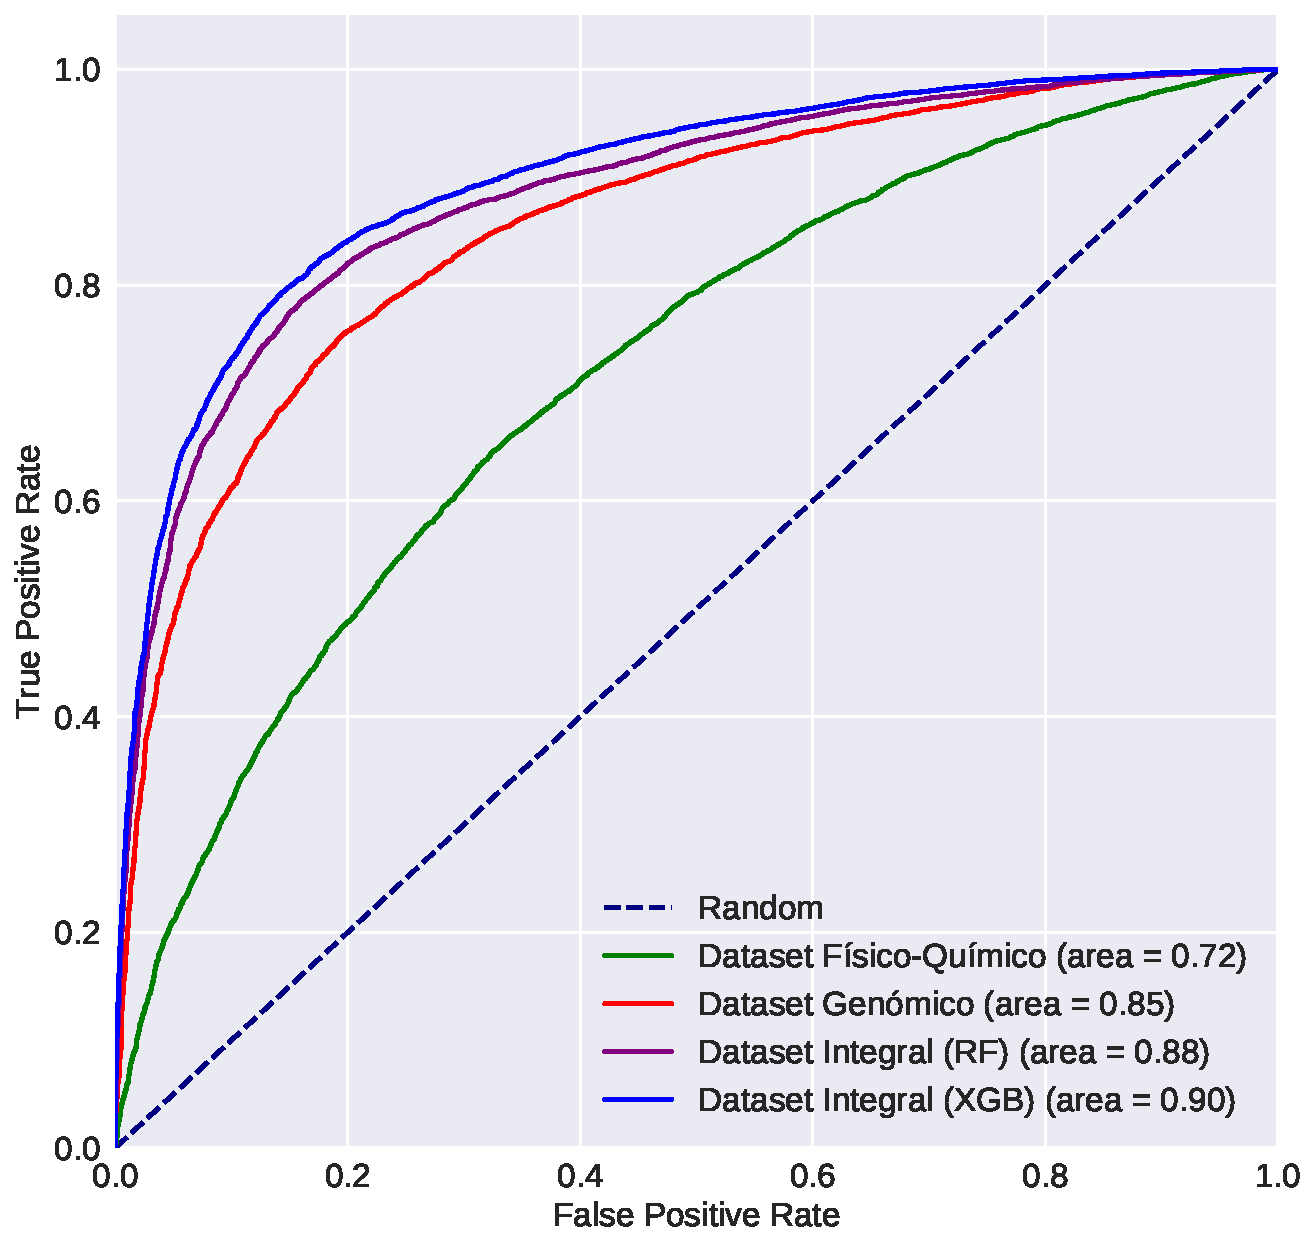
\includegraphics[width=\textwidth]{documents/latex/figures/4/curvas_auc_humsavar.pdf}
    \caption{Comparación de curvas ROC entre los datasets Físico-Químico, Genómico e Integral.}
    \label{fig:curvas_auc_humsavar}
\end{subfigure}

\hfill
\hfill

\begin{subfigure}[b]{0.6\textwidth}
    \centering
    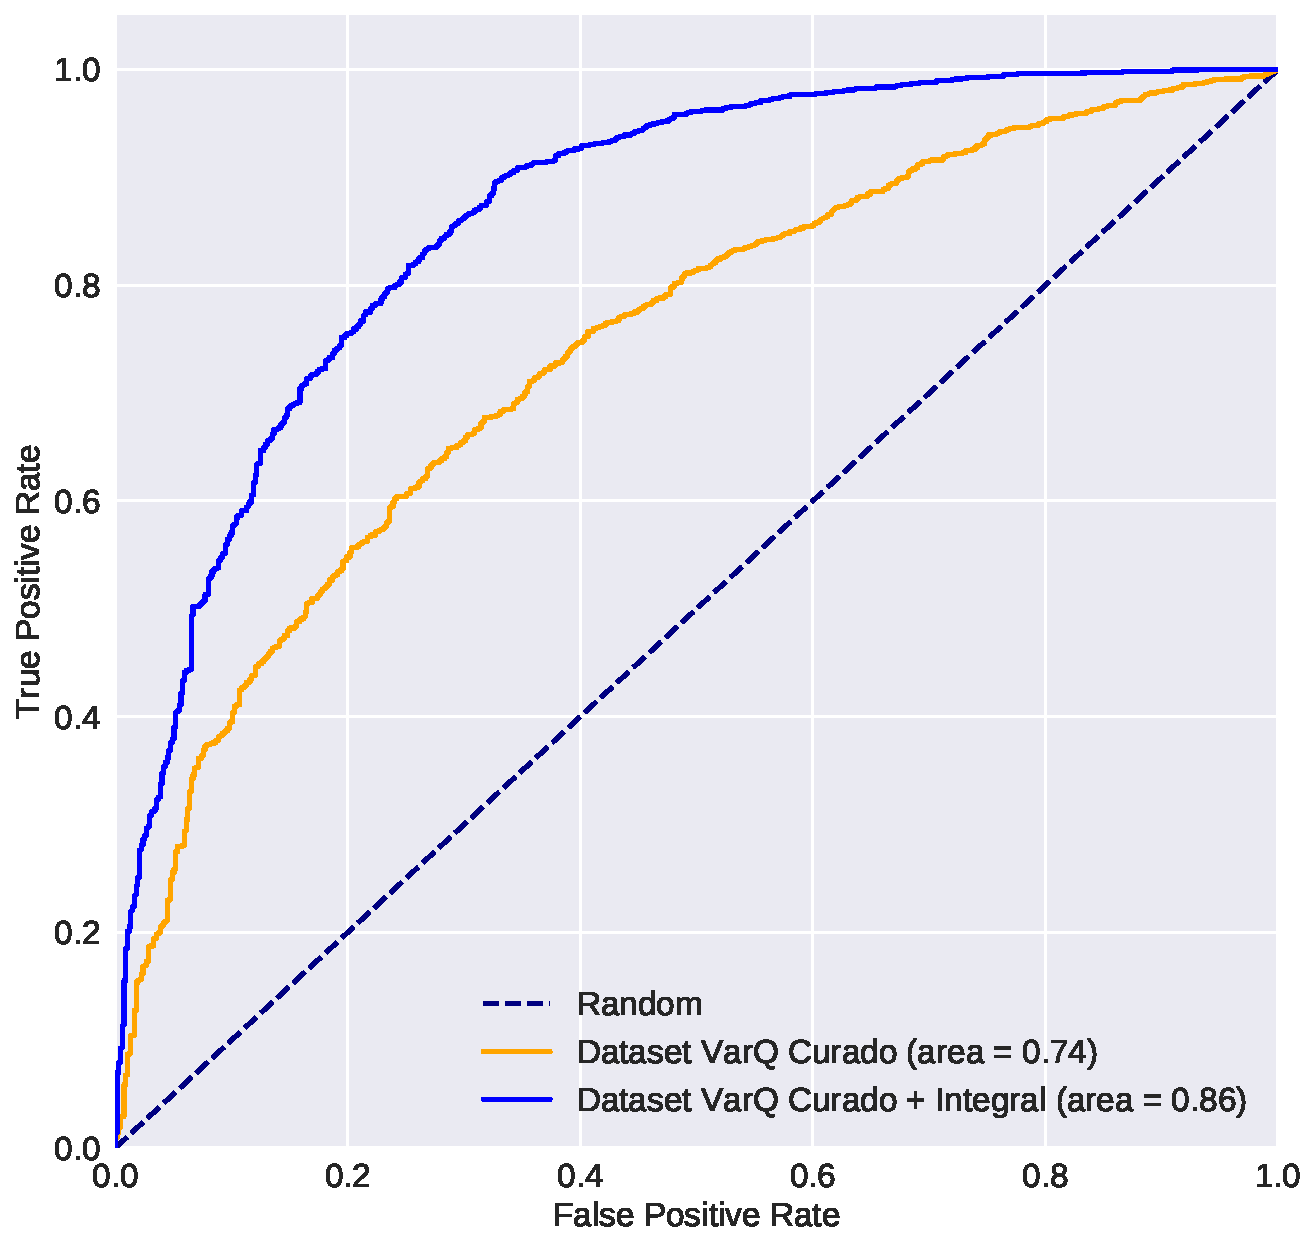
\includegraphics[width=\textwidth]{documents/latex/figures/4/curvas_auc_varq.pdf}
    \caption{Comparación de curvas ROC entre los datasets VarQ Curado y VarQ Curado + Integral.}
    \label{fig:curvas_auc_varq}
\end{subfigure}

\caption{Comparación de curvas AUC usando datasets con variantes de Humsavar y VarQ Curado.}
\end{figure}




% \chapter{Apéndice}
% \label{ch:apendice}
% \section{Estructura del proyecto}

A continuación detallamos los distintos módulos del proyecto para facilitar la replicación de los resultados obtenidos. Este se encuentra alojado en GitHub. 

El proyecto tiene la siguiente estructura:

\vspace{0.2cm}
\dirtree{%
.1 master-thesis.
.2 data.
.2 notebooks.
.2 results.
.3 varq.
.3 physico\_chemical.
.3 genomic.
.3 integral.
.3 varq\_integral.
.2 src.
.3 snvbox\_queries.
}
\vspace{0.2cm}

En \texttt{src} se encuentra el código necesario para obtener las variables de la tabla SNVbox y generar las variables a partir de la data externa (por ejemplo, Humsavar) que se encuentra en la carpeta \texttt{data}. Luego, para cada modelo existe una notebook para generar el dataset y otro para evaluar los algoritmos, que almacenan los resultados en \texttt{results}. 


\section{Diccionario de hiperparámetros usados}

Para los modelos usados, se usaron los siguientes diccionarios de parámetros:
\begin{itemize}
    \item Random Forest
        \begin{itemize}
            \item Profundidad del árbol: [3, 5, 7]
            \item Estimadores: [10, 50, 100]
            \item Cantidad de variables por árbol: [4, $\sqrt{n}$, $0.2*n$] con n la cantidad total de variables
        \end{itemize} 
    \item Regresión logística:
        \begin{itemize}
            \item Parámetro de regularización inverso (C): [.001, .01, .1, 1, 10, 100, 1000]
            \item Peso de las clases: [balanceado, igual a 1]
        \end{itemize}
    \item SVC:
        \begin{itemize}
            \item Parámetro de penalidad (C): [0.001, 0.10, 0.1, 10, 25, 50, 100, 1000]
            \item Gamma: [0.001, 0.10, 0.1, 10, 25, 50, 100, 1000]
        \end{itemize}
    \item XGBoost:
        \begin{itemize}
            \item Peso mínimo de las hojas: [1, 5, 10]
            \item Gamma: [0.5, 1, 1.5, 2, 5]
            \item Subsample: [0.6, 0.8, 1.0]
            \item colsample\_bytree: [0.6, 0.8, 1.0]
            \item Profundidad máxima: [3, 4, 5]
        \end{itemize}
\end{itemize}


\section{Lista de Variables de SNVBox}

\subsubsection{Variables sobre cambios en la sustitución del Aminoácido (Estructura Primaria)}
\begin{itemize}
    \item Score BLOSUM (AABLOSUM): Score de la matriz BLOSUM 62.
    \item Carga (AACharge): El cambio en la carga resultante de cambiar el aminoácido de referencia con la mutación.
    \item Volumen (AAVolume): El cambio en el residuo resultante del cambio de aminoácido (expresado en Angstroms cúbicos).
    \item Hidrofobia (AAHydrophobicity): El cambio en hidrofobicidad resultante de la mutación.
    \item Score Grantham (AAGrantham): La distancia Grantham de la referencia a la mutación.
    \item Polaridad (Polarity): Cambio de polaridad entre la referencia y la mutación.
    \item Score Ex (AAEx): Score de la matriz EX.
    \item Score PAM250 (AAPAM250): Score de la matriz PAM250.
    \item Score MJ (AAMJ): Score de la matriz Miyagawa-Jerningan.
    \item Score HGMD2003 (AAHGMD2003): Número de veces que la sustitución ocurre en la base de datos HGMD.
    \item Score VB (AAVB): Score de la matriz VB (Venkatarajan \& Braun).
    \item Transición (Transition): Frecuencia de la transición entre dos aminoácidos vecinos basado en todas las proteínas de SwissProt/TrEMBL.
    \item COSMIC: Frecuencia de cambio \textit{missense} en la base COSMIC.
    \item COSMICvsSWISSPROT: Frecuencia de cambio \textit{missense} sobre la cantidad de proteínas en SwissProt.
    \item HAPMAP: Cantidad de sustituciones en HAPMAP.
    \item COSMICvsHAPMAP: Frecuencia de cambio \textit{missense} sobre la cantidad de proteínas en HAPMAP.
\end{itemize}

\subsubsection{Variables a nivel de Proteína (sin considerar sustitución)}

\begin{itemize}
    \item BINDING: Sitio de unión.
    \item ACTIVE\_SITE: Actividad enzimática. 
    \item SITE: Sitio ``interesante''.
    \item LIPID: Unión con un lípido.
    \item METAL: Unión con un metal.
    \item CARBOHYD: Unión con un carbohidrato.
    \item DNA\_BIND: Unión con ADN.
    \item NP\_BIND: Unión con un nucleótido fosfato.
    \item CA\_BIND: Unión con calcio.
    \item DISULFID: Sitio de unión con un disulfuro.
    \item SE\_CYS: Selenocisteína.
    \item MOD\_RES: Residuo modificado.
    \item PROPEP: Propéptido.
    \item SIGNAL: Sitio de señal de localización.
    \item TRANSMEM: Proteína transmembranal.
    \item COMPBIAS: Sesgo de composición.
    \item REP: Región de repetición.
    \item MOTIF: Sitio de un motif funcional conocido.
    \item ZN\_FING: Dedo de zinc.
    \item REGIONS: Región de interés en la secuencia proteica.
    \item PPI: Interacción proteína-proteína.
    \item RNABD: Unión RNA.
    \item TF: Factor de transcripción. 
    \item LOC: Sitio que determina correcta localización celular de una proteína. 
    \item MMBRBD: Sitio que se une a la membrana celular.
\end{itemize}

% \vspace{2mm}
% \todo{
% TODO:
% Diagrama de SNVBOX
% }
% \vspace{2mm}



%%%% BIBLIOGRAFIA

\backmatter

\bibliography{references/reference}
\addcontentsline{toc}{chapter}{Bibliografía}

\bibliographystyle{abbrv}



\end{document}
